\documentclass{article}
\title{Web-based Supplementary Materials for Combinatorial Mixture Models for Single-Cell Assays with Application to Vaccine Studies by Greg Finak, Steve De Rosa, Mario Roederer and Raphael Gottardo}

\usepackage[margin=1in]{geometry}
\usepackage{amssymb}
\usepackage{booktabs}
\usepackage{multirow,natbib}
\usepackage{url}
\def\bSig\mathbf{\Sigma}
\newcommand{\VS}{V\&S}
\newcommand{\tr}{\mbox{tr}}
\usepackage{amsmath,tikz}
\usetikzlibrary{calc}
\usetikzlibrary{positioning}
\date{}
\begin{document}
\maketitle
\appendix
%\renewcommand{\thesection}{\Alph{section}}
\renewcommand{\thesubsection}{Web Appendix \Alph{subsection}:}
%\setcounter{section}{1}
\setcounter{subsection}{0}
%\setcounter{figure}{0}
\renewcommand{\figurename}{\textbf{Web Figure}}
\renewcommand{\thefigure}{\textbf{\Alph{figure}}}
\setcounter{figure}{0}
%\todo[inline]{Note that the Supplementary Information section needs corrections to notation and overall}

\section*{}
\subsection{HVTN065 vaccine trial ICS data description}
\label{supp:statpublished}
HVTN065 is a phase 1 (safety and immunogenicity) trial of GeoVax HIV/AIDS DNA and MVA vaccine in 120 individuals (100 vaccinees, 20 placebo recipients, parts A and B). CD4 and CD8 T--cell epitope specific immune responses were measured via the ICS assay. 
% No need to talk about this
% Other humoral and cellular immune responses were measured via ELISA, and neutralizing antibody assays. 
Cytokines measured in the ICS assay included IFNg, TNFa, IL2, and IL4, and antigens included three Env, three Gag, and three Pol peptide pools. Results of the trial have been published in \cite{Goonetilleke:2006jk}.

%HVTN054 is a phase 1 (safety and immunogenicity) trial of an adenoviral vector vaccine in individuals without prior immunity~\cite{Peiperl:2010ej}. The vaccine vector expressed Gag, Pol and Env proteins from multiple HIV clades~\cite{Peiperl:2010ej}. Vaccine was given at two increasing doses, as well as a placebo. T--cell responses to antigens in the vaccine were measured via the ICS assay~\cite{Peiperl:2010ej,Horton:2007tsa}. The cytokines measured were IFNg (Interferon--$\gamma$), IL2 (Interleukin--2), TNFa (Tumor necrosis factor--$\alpha$) and IL4 (Interleukin 4)~\cite{Horton:2007tsa}. The sample size consisted of 20 vaccine and four placebo recipients. The original statistical analysis of the positivity calls is described in the associated publication~\cite{Peiperl:2010ej}. The Gag stimulated, IL2 expressing, CD4+ T--cell data from day 28 was used to derive hyper--parameter estimates for the simulation studies. 
\subsection{Computational details for the beta-binomial model}
\noindent\textbf{Marginal likelihood derivations}\\
\noindent\textbf{MCMC algorithm}\\
In what follows, we use $(x|y)$ to denote the conditional distribution of $x$ given $y$. In particular, we use $(x|\cdots)$ to denote the distribution of $x$ conditional on everything else in the model. Our MCMC algorithms cycle through the following steps: 
\begin{enumerate}
\item Update each $\alpha_u, \beta_u, \alpha_s$ and $\beta_s$ by Metropolis-Hastings using a Gaussian symmetric proposal where the variance of the proposal is tune for each parameter using the approach of (Greg add the citation).
\item Update $w$ by Gibbs sampling using the full conditional,
\[
(w|\cdots)\sim
\]
\item for each $i$, update $z_i$ by Gibbs sampling using the following full conditional,
\[
(z_i|\dots)\sim
\]
\end{enumerate}
For each updated parameter, step 1 above involves the calculation of the following acceptance ratio
\[
add\ formula.
\]
where $\pi$ is the prior distribution of the corresponding parameter. In our case each parameter has the same exponential prior with mean $10^3$\footnote{Check that this is correct}.
\subsection{Constrained beta--binomial model}
\label{supp:constrained}
We can define a model where we constrain the stimulated proportions under the alternative model such that $p_s>p_u$. In this case, the only changes required are for the alternative marginal likelihood $\mathrm{L}_1$ defined in the main manuscript by (1). Due to the constraint, the normalizing constant of the prior under the alternative (model ${\cal M}_1$) is not given by $\mathrm{B}(\alpha_u,\beta_u)\mathrm{B}(\alpha_s,\beta_s)$ but requires computing \[
Z(\alpha_u, \beta_u, \alpha_s, \beta_s)=\int_{0}^1{p_u}^{\alpha_u-1}(1-p_u)^{\beta_u-1}\int_{p_u}^1 p_s^{\alpha_s-1}(1-p_s)^{\beta_s-1}dp_sdp_u.
\]
Using this expression, the constrained alternative marginal likelihood can be written as 
\begin{align}
	\begin{split}
\mathrm{L}_1(\alpha_u,\beta_u,\alpha_s,\beta_s|\mathbf{y}) 
=&\prod_{i=1}^P\binom{N_{ui}}{n_{ui}} \binom{N_{si}}{n_{si}}\cdot\\ &\frac{Z(n_{ui}+\alpha_u,N_{ui}-n_{ui}+\beta_u,n_{si}+\alpha_s,N_{si}-n_{si}+\beta_s)}{Z(\alpha_u,\beta_u,\alpha_s,\beta_s)}.\\
\label{model2:constrained}
\end{split}
\end{align}


In general, there is no closed form expression for $Z(\cdot)$, and a numerical approximation must be used. Let us denote by $\tilde{Z}(\alpha_u, \beta_u, \alpha_s, \beta_s)$ the approximation. A natural way to estimate $\tilde{Z}$ is to use Monte Carlo integration. Indeed, we can write 
\begin{equation}
\tilde{Z}(\alpha_u, \beta_u, \alpha_s, \beta_s)=\mathrm{B}(\alpha_u,\beta_u)\mathrm{B}(\alpha_s,\beta_s)\int_{0}^1\frac{{p_u}^{\alpha_u-1}(1-p_u)^{\beta_u-1}}{\mathrm{B}(\alpha_u,\beta_u)}(1-F_{\alpha_s,\beta_s}(p_u))dp_u
\label{equ:normZ}
\end{equation}
where $F_{\alpha_s,\beta_s}$ is the cumulative distribution function of a beta random variable with parameters $\alpha_s$ and $\beta_s$. Using this identity, it can be seen that $\tilde{Z}(\alpha_u, \beta_u, \alpha_s, \beta_s)$ can be approximated by 
\[
\tilde{Z}(\alpha_u, \beta_u, \alpha_s, \beta_s)\approx\mathrm{B}(\alpha_u,\beta_u)\mathrm{B}(\alpha_s,\beta_s)\sum_{k=1}^K(1-F_{\alpha_s,\beta_s}(X_k))
\]
where the $X_k$'s are \textit{iid} beta distributed random variables with parameters $\alpha_s$, $\beta_s$ and $K$ is the number of terms used in the Monte Carlo approximation. This approximation works relatively well with our EM implementation and does not significantly increase the computing time.
Unfortunately, the number of terms (\textit{i.e.} value of $I$) required for the approximation to be good might be large and computing such a normalizing constant at each iteration would significantly slow down our MCMC implementation. As it tuns out, a better approximation
can be obtained when $\alpha_s$ and $\beta_s$ are integers. In this case, the cdf function in \eqref{equ:normZ} can be calculated exactly using integration by parts, as follows,
\[
F_{\alpha_s,\beta_s}(p_u)=\sum_{j=\beta_s}^{\beta_s+\alpha_s-1} \frac{(\beta_s+\alpha_s-1)!}{j!(\beta_s+\alpha_s-j)!}(1-p_u)^jp_u^{\beta_s+\alpha_s-j}.
\label{eq:IBident}
\]
Then using, this identity, we obtain
\begin{align*}
Z(\alpha_u, \beta_u, \alpha_s, \beta_s)&=\mathrm{B}(\alpha_s,\beta_s)\sum_{j=\beta_s}^{\beta_s+\alpha_s-1}\frac{(\beta_s+\alpha_s-1)!}{j!(\beta_s+\alpha_s-j)!}\int_{0}^1(1-p_u)^{\beta_u-1+j}p_u^{\alpha_u-1+\beta_s+\alpha_s-j}dp_u\\
&=\mathrm{B}(\alpha_s,\beta_s)\sum_{j=\beta_s}^{\beta_s+\alpha_s-1}\frac{(\beta_s+\alpha_s-1)!}{j!(\beta_s+\alpha_s-j)!}\mathrm{B}(\beta_u+j)\mathrm{B}(\alpha_u+\beta_s+\alpha_s-j).
\label{equ:normZ}
\end{align*}
Typically, in ICS data $\alpha_s$ is relatively small leading to relatively few terms in the sum. However, the use of this exact identity in our MCMC algorithm requires the use of discrete priors on $\alpha_s$ and $\beta_s$, which can be restrictive in terms of fit (\textit{e.g.},  if the true $\alpha_s$ is less than one) and can render mixing in the MCMC more difficult. In addition, even though the computation is exact and much faster for small values of $\alpha_s$, which is typically the case with ICS data, it is still more demanding than the unconstrained model. In our case, we have decided to use the unconstrained model and simply fix the $z_i$ to zero if the empirical proportion for the un-stimulated sample, $p_u$, is less than that of the stimulation sample, $p_s$. Indeed, in the one-sided case, if $p_u>p_s$ the associated individual should be a non-responder and thus $z_i=0$. In our experience, this computational shortcut performs just as well as the true one-sided implementation while being computationally much less demanding.  

\subsection{Computational details for the Dirichlet-multinomial model}
\noindent\textbf{Marginal likelihood derivations}\\
Because our Dirichlet-multinomial is a direct extension of the beta-binomial model, the marginal likelihoods are obtained in the exact same fashion.The derivations is described below,

\noindent\textbf{MCMC algorithm}\\
GREG: Look at the what I did above, and do something similar here.
\begin{figure} %  figure placement: here, top, bottom, or page
   \centering
%   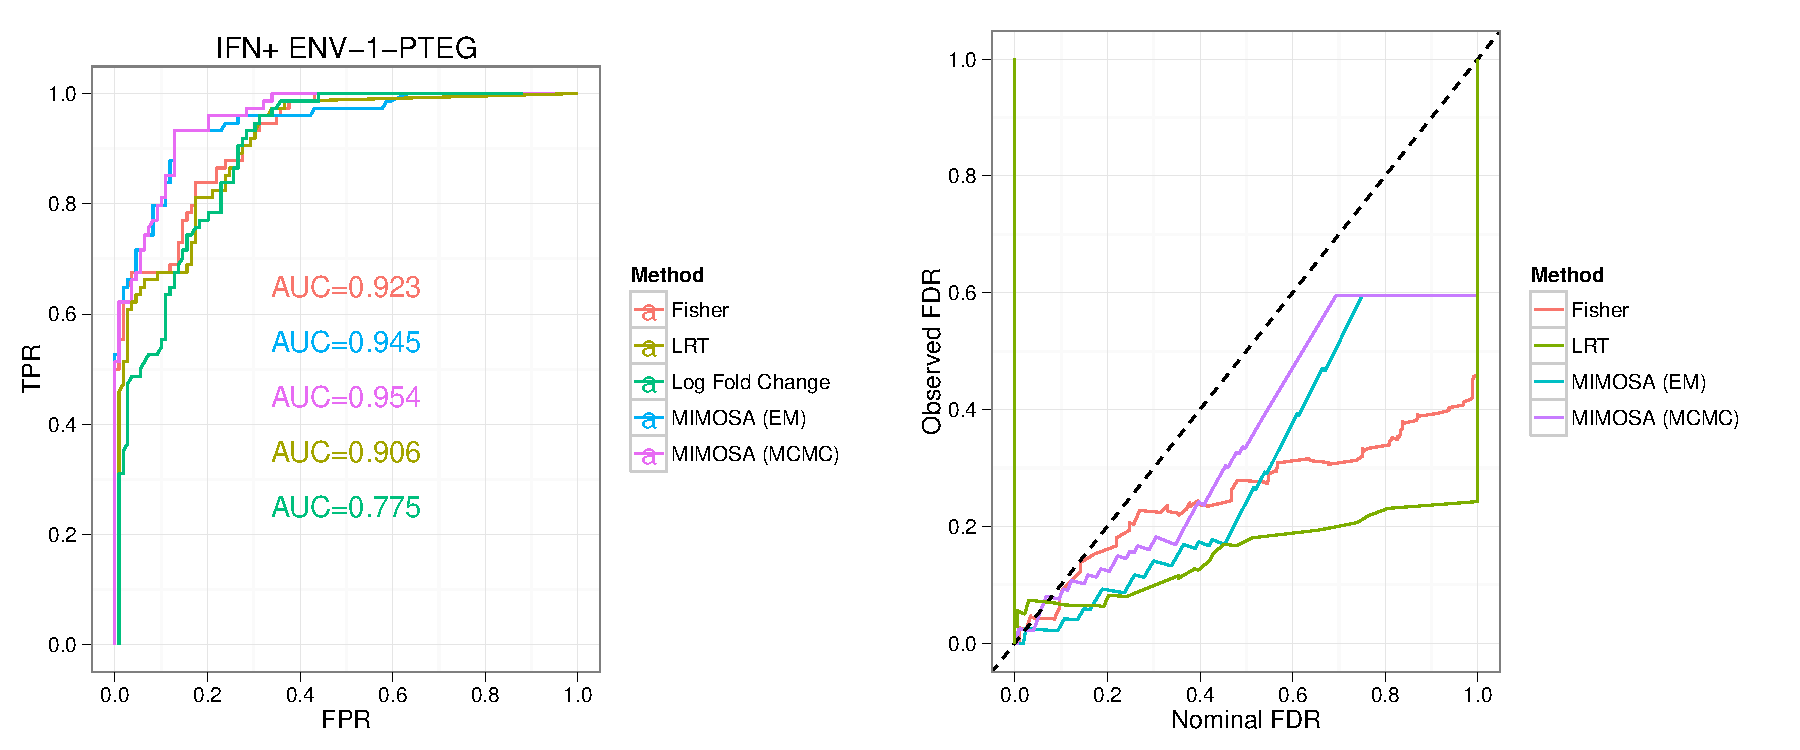
\includegraphics[width=.75\columnwidth]{Figures/2}\\ 
%   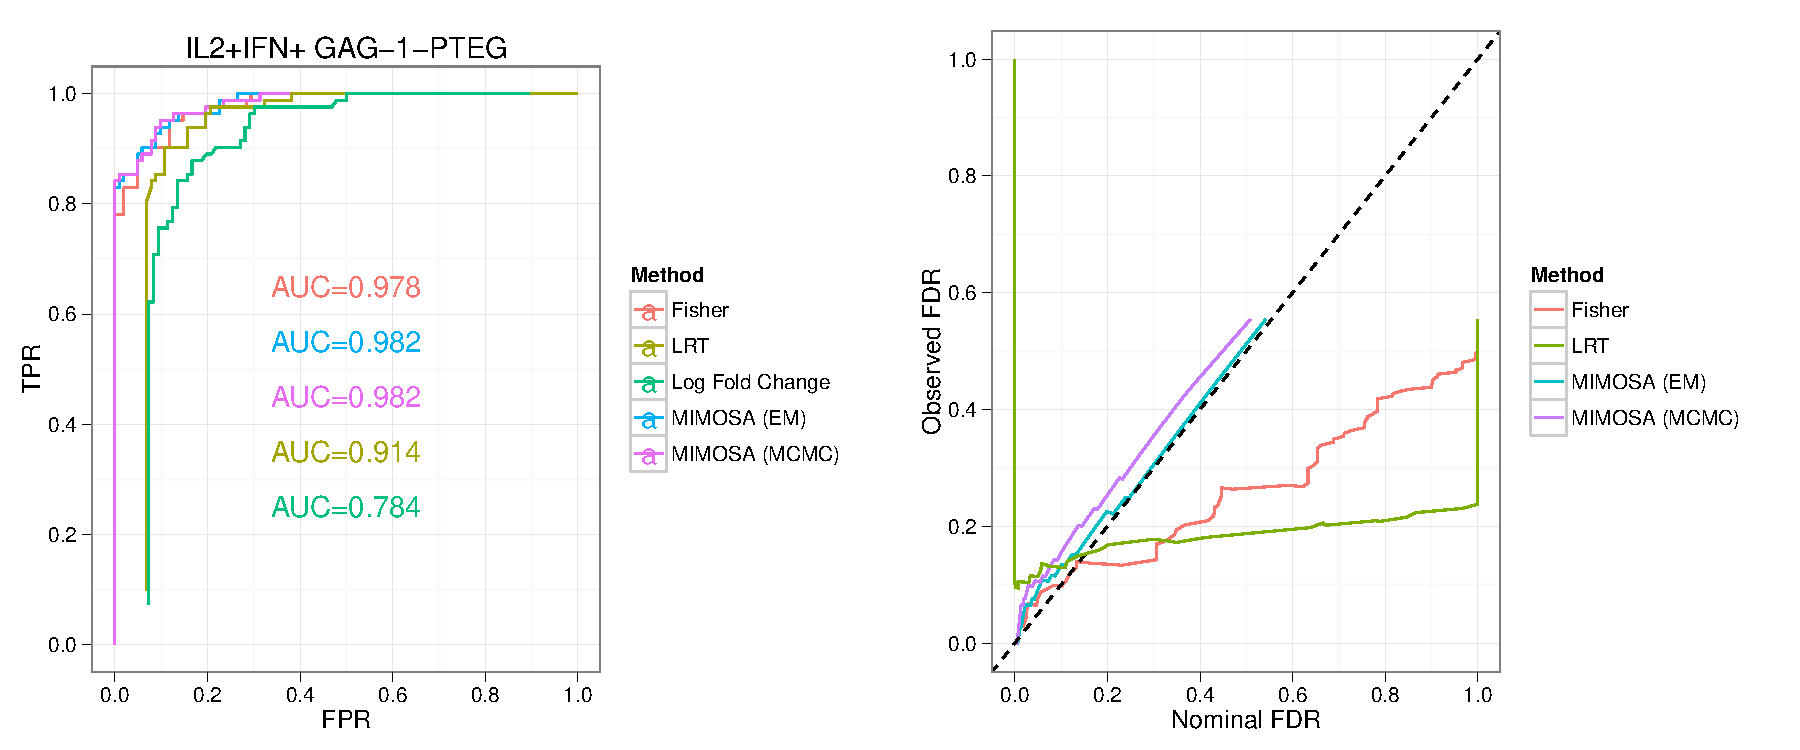
\includegraphics[width=.75\columnwidth]{Figures/12} 
\begin{tikzpicture} [auto, node distance=0cm]
\node at (0,0) (A){
\begin{tikzpicture}
    \node[anchor=south west,inner sep=0] at (0,0) (a) {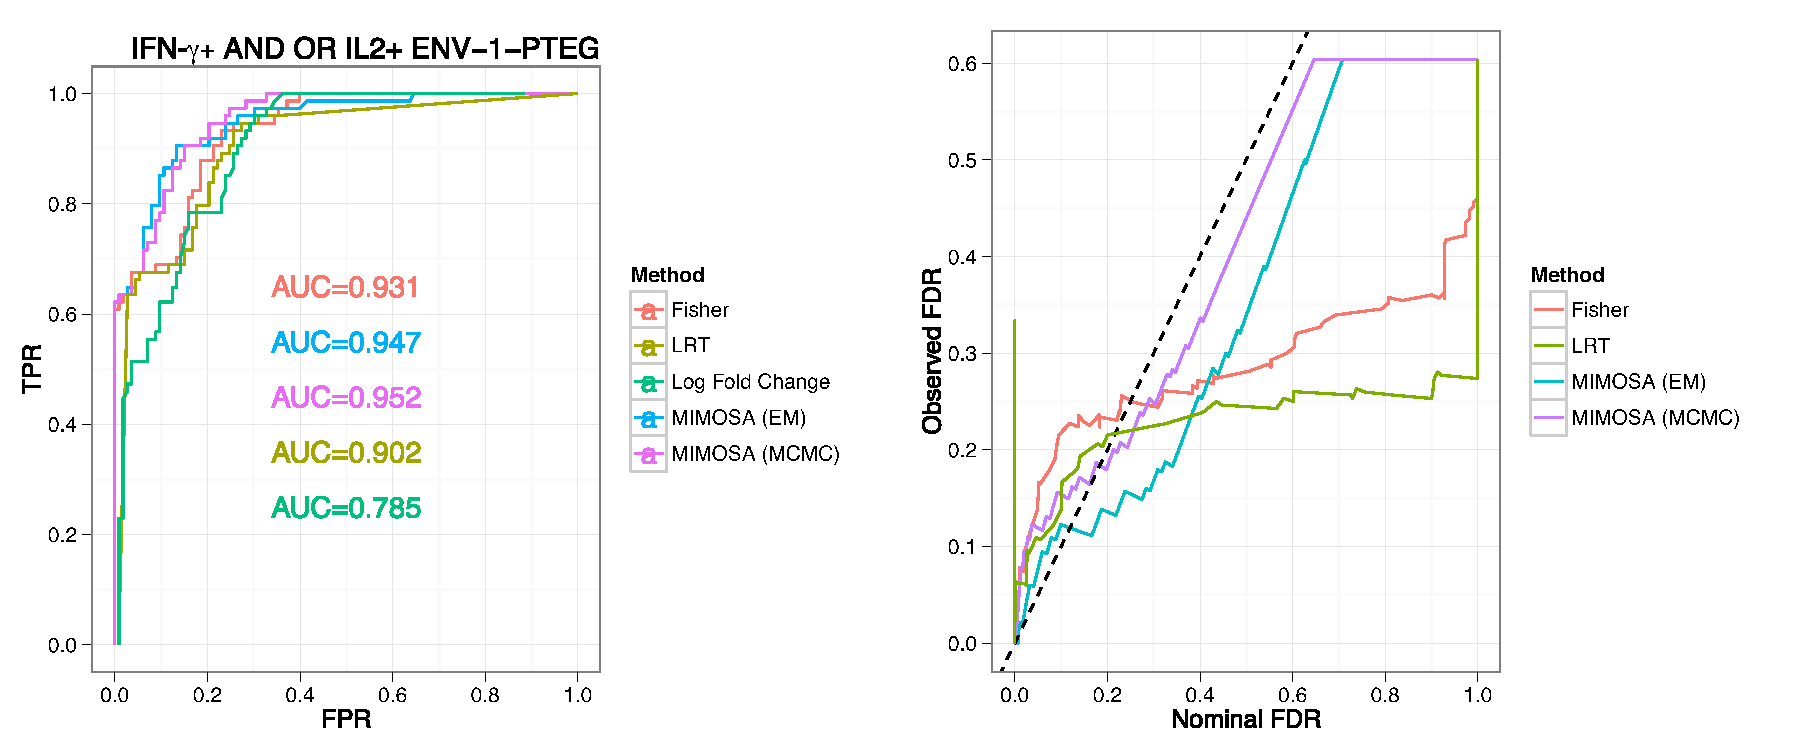
\includegraphics[width=.5\columnwidth]{Figures/15}};
    \begin{scope}[x={(a.south east)},y={(a.north west)}]
        \node at (0,1) [font=\small\sffamily] {A} ;
        \end{scope}
        \end{tikzpicture}
 };
 \node [right=of A] (B) {
 \begin{tikzpicture}
    \node[anchor=south west, inner sep=0] at (0,0) (b) {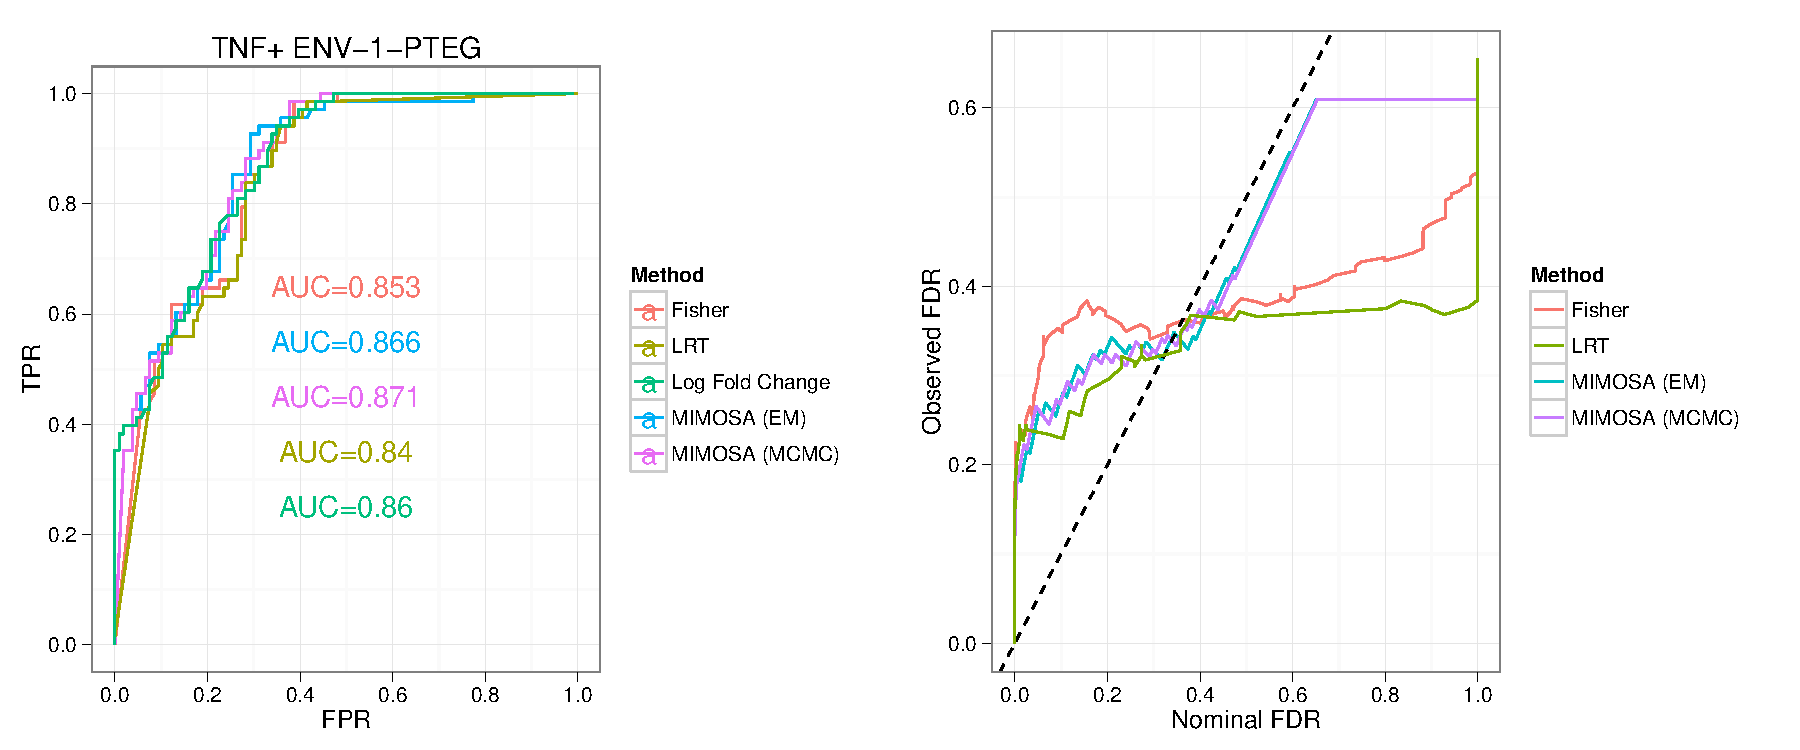
\includegraphics[width=.5\columnwidth]{Figures/3}};
        \begin{scope}[x={(b.south east)},y={(b.north west)}]
        \node at (0,1) [font=\small\sffamily] {B} ;
                \end{scope}
        \end{tikzpicture}
 };
 \node [below=of A] (C) {
 \begin{tikzpicture}
    \node[anchor=south west, inner sep=0] at (0,0) (c) {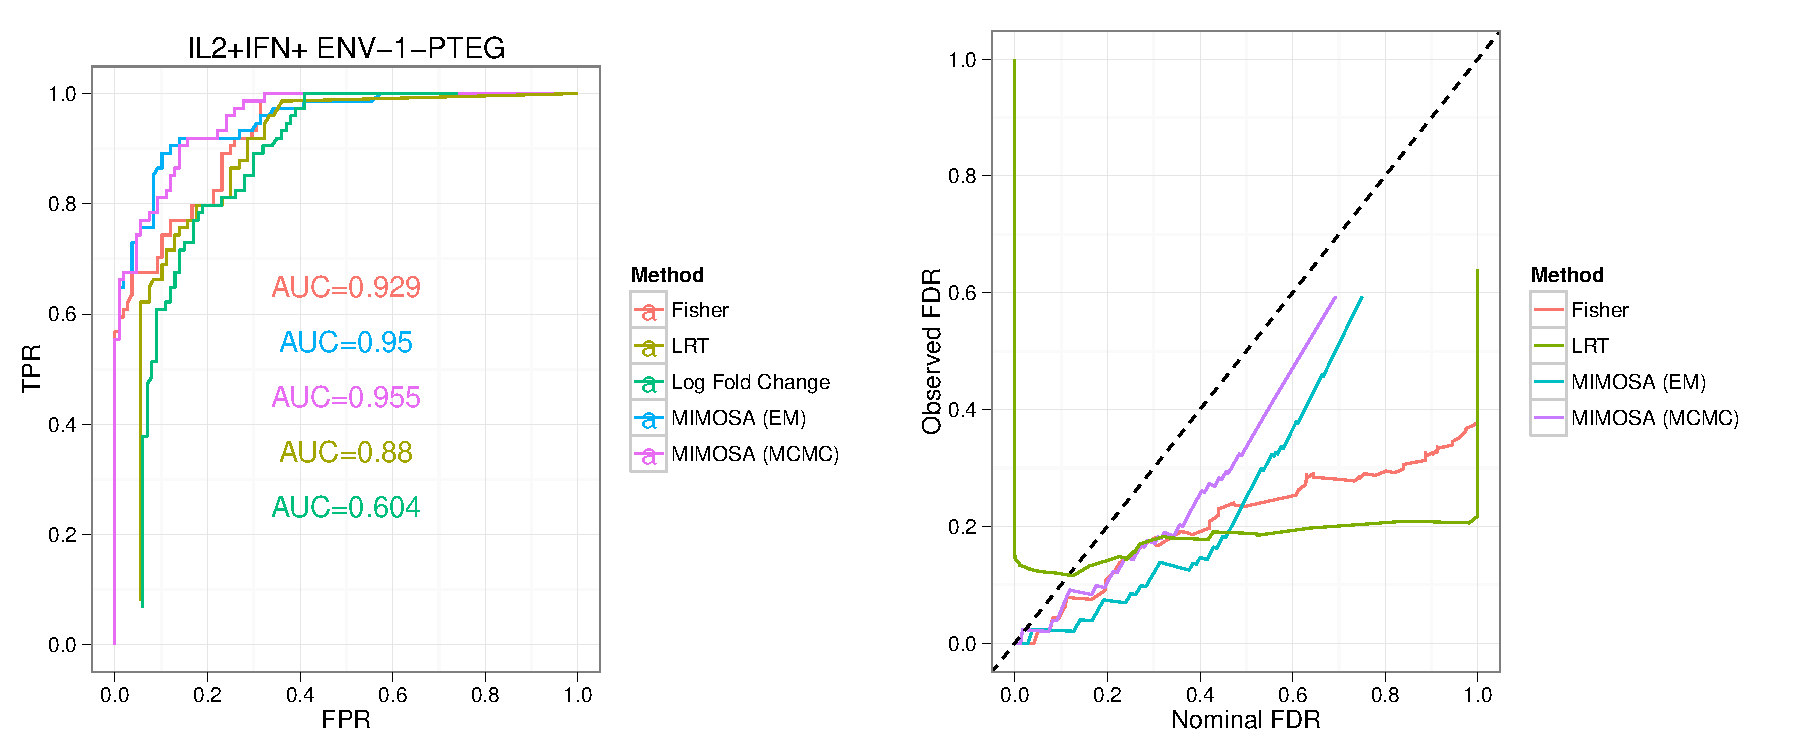
\includegraphics[width=.5\columnwidth]{Figures/5}};
        \begin{scope}[x={(c.south east)},y={(c.north west)}]
        \node at (0,1) [font=\small\sffamily] {C} ;
        \end{scope}
        \end{tikzpicture}
};
\node [below=of B] (D) {
\begin{tikzpicture}
    \node[anchor=south west, inner sep=0] at (0,0) (d) {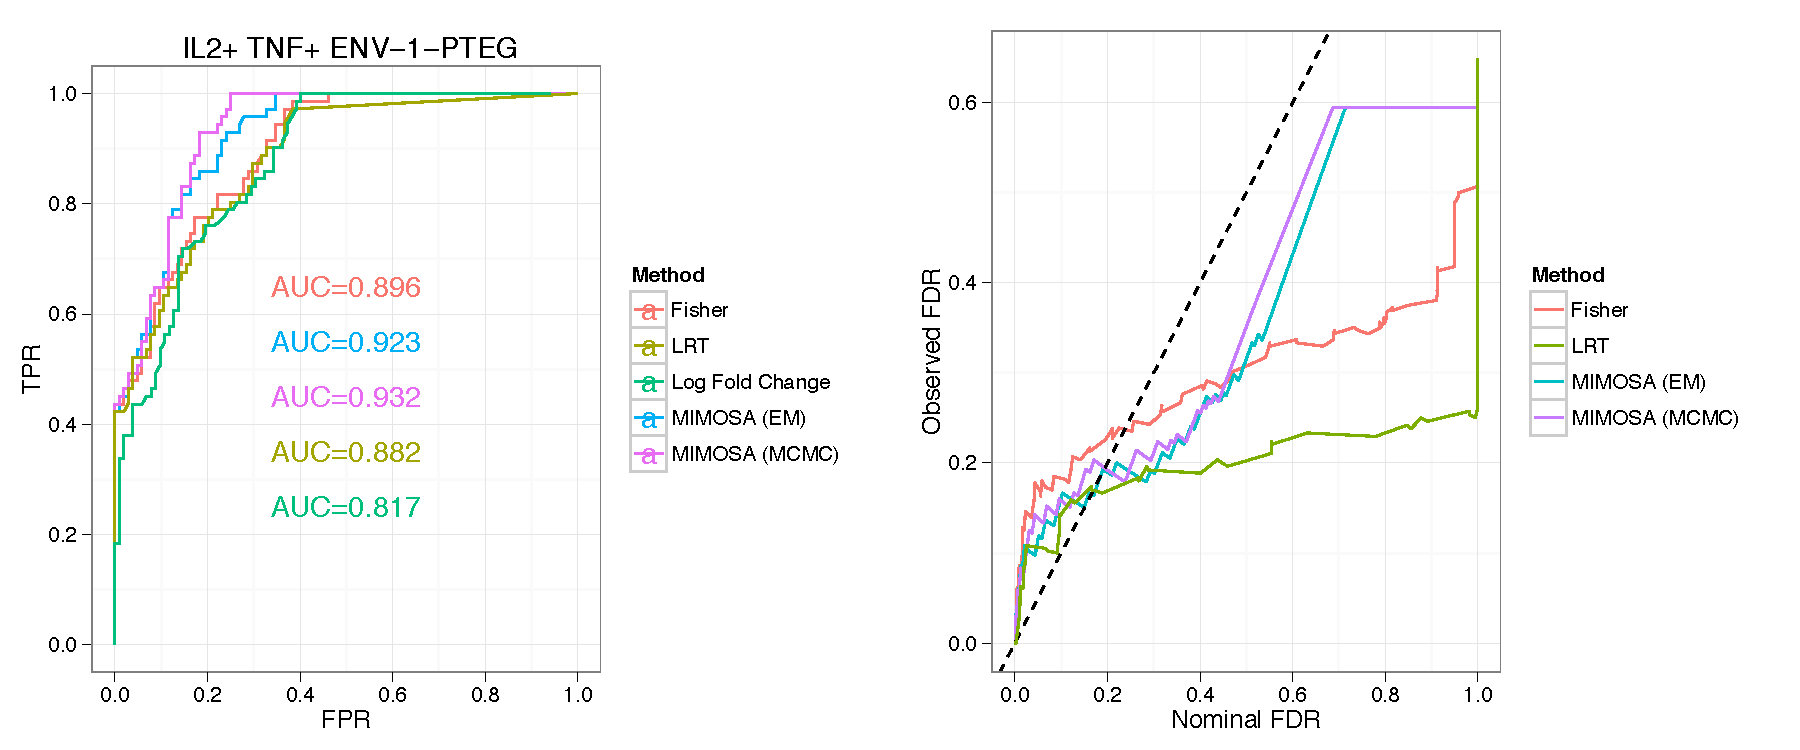
\includegraphics[width=.5\columnwidth]{Figures/6}};
        \begin{scope}[x={(d.south east)},y={(d.north west)}]
        \node at (0,1) [font=\small\sffamily] {D} ;
                \end{scope}
        \end{tikzpicture}
};
\node [below=of C] (E) {
\begin{tikzpicture}
    \node[anchor=south west, inner sep=0] at (0,0) (e) {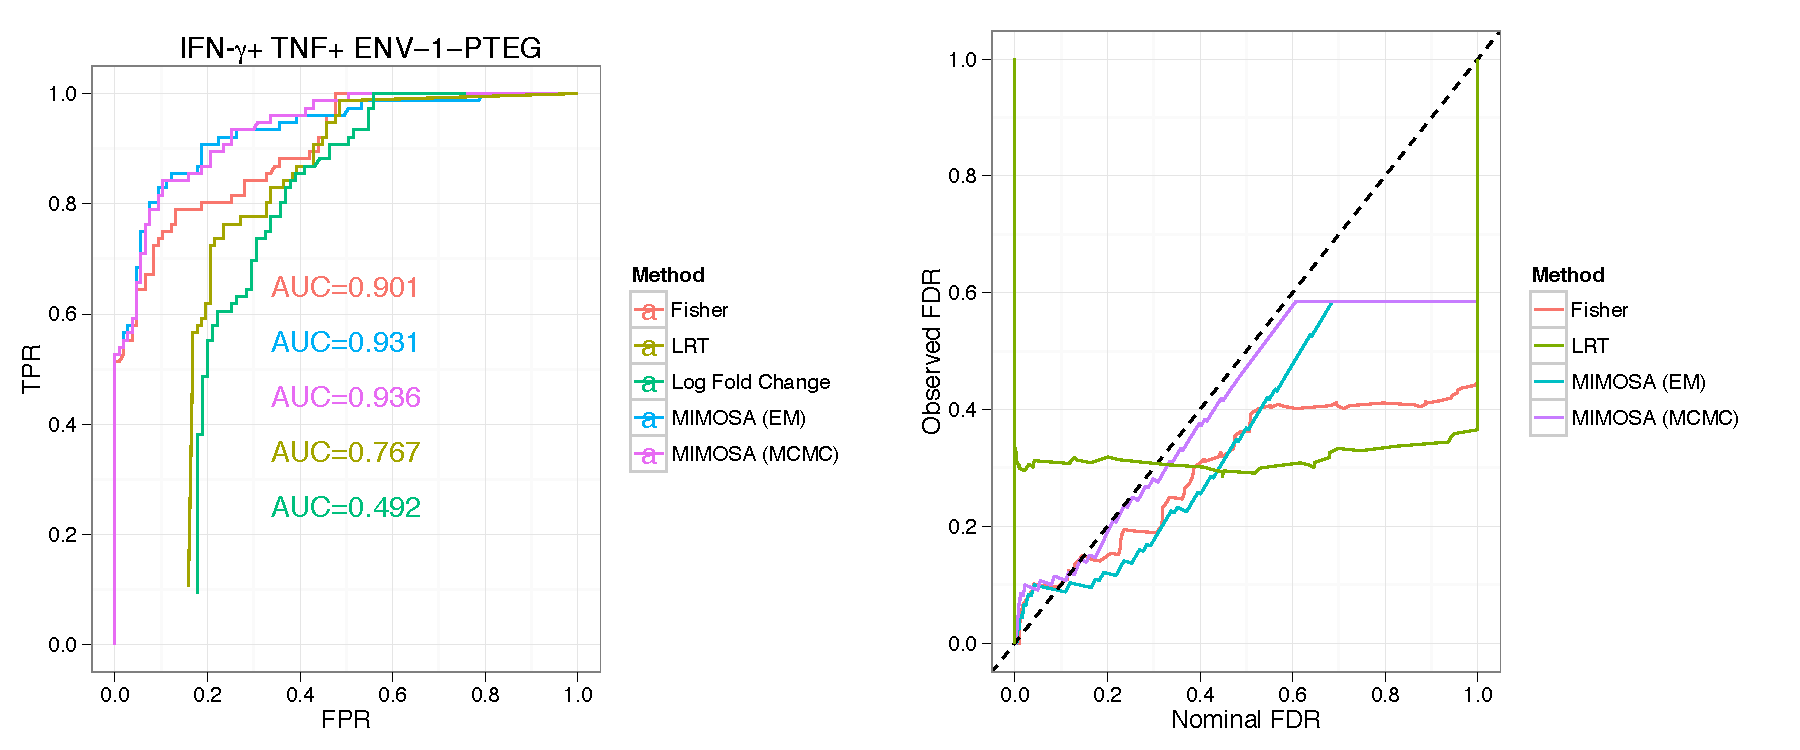
\includegraphics[width=.5\columnwidth]{Figures/7}};
        \begin{scope}[x={(d.south east)},y={(d.north west)}]
        \node at (0,1) [font=\small\sffamily] {E} ;
                \end{scope}
        \end{tikzpicture}
 };
   % \node[anchor=south west, inner sep=0] at (8,-7.5){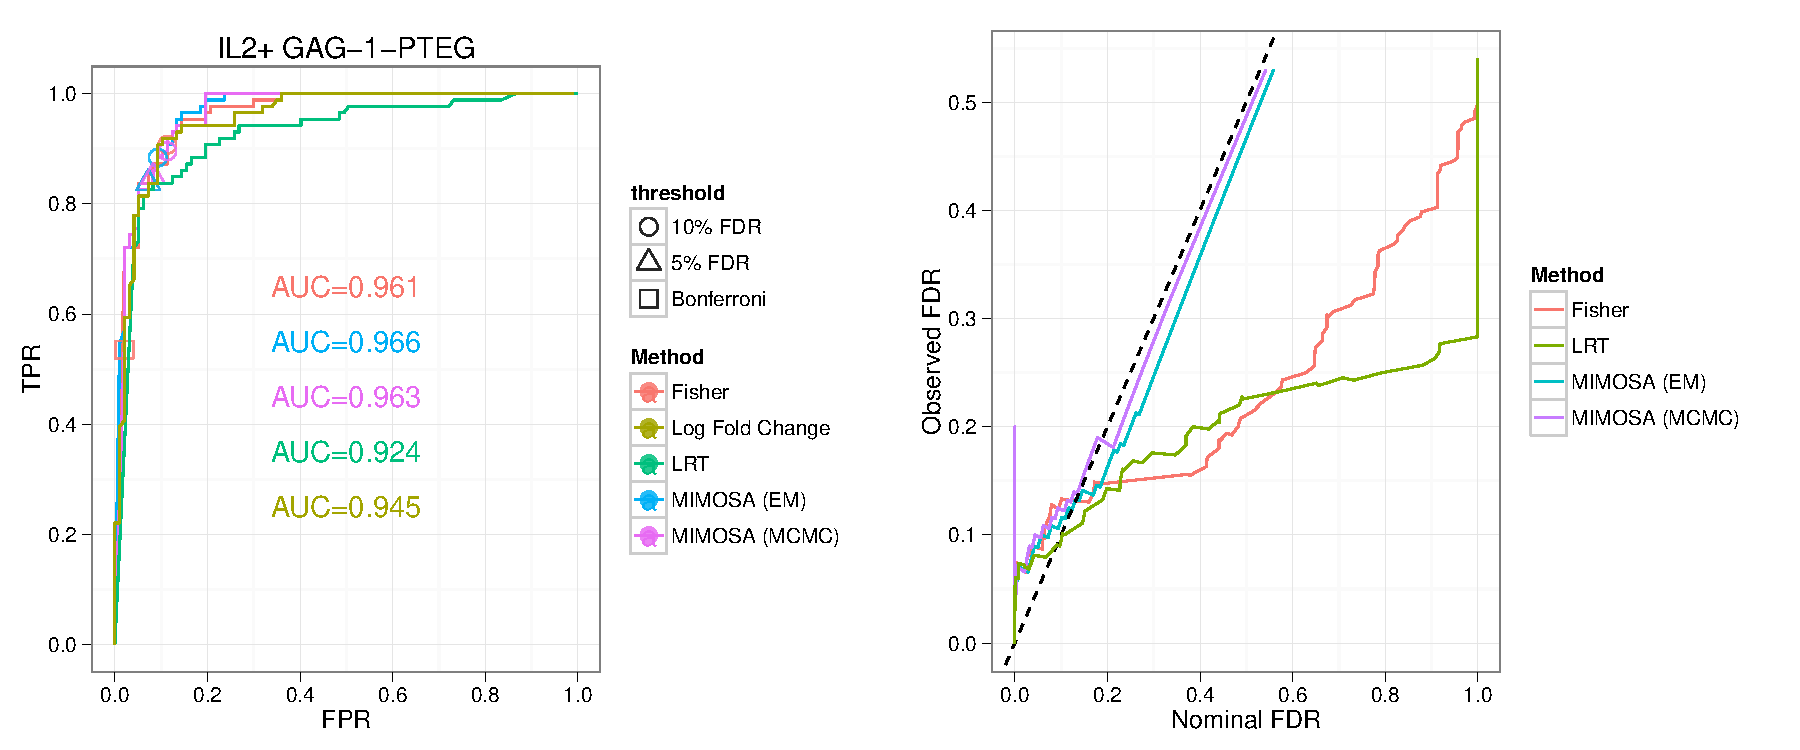
\includegraphics[width=.5\columnwidth]{Figures/8}};
   % \node[anchor=south west, inner sep=0] at (0,-11.25){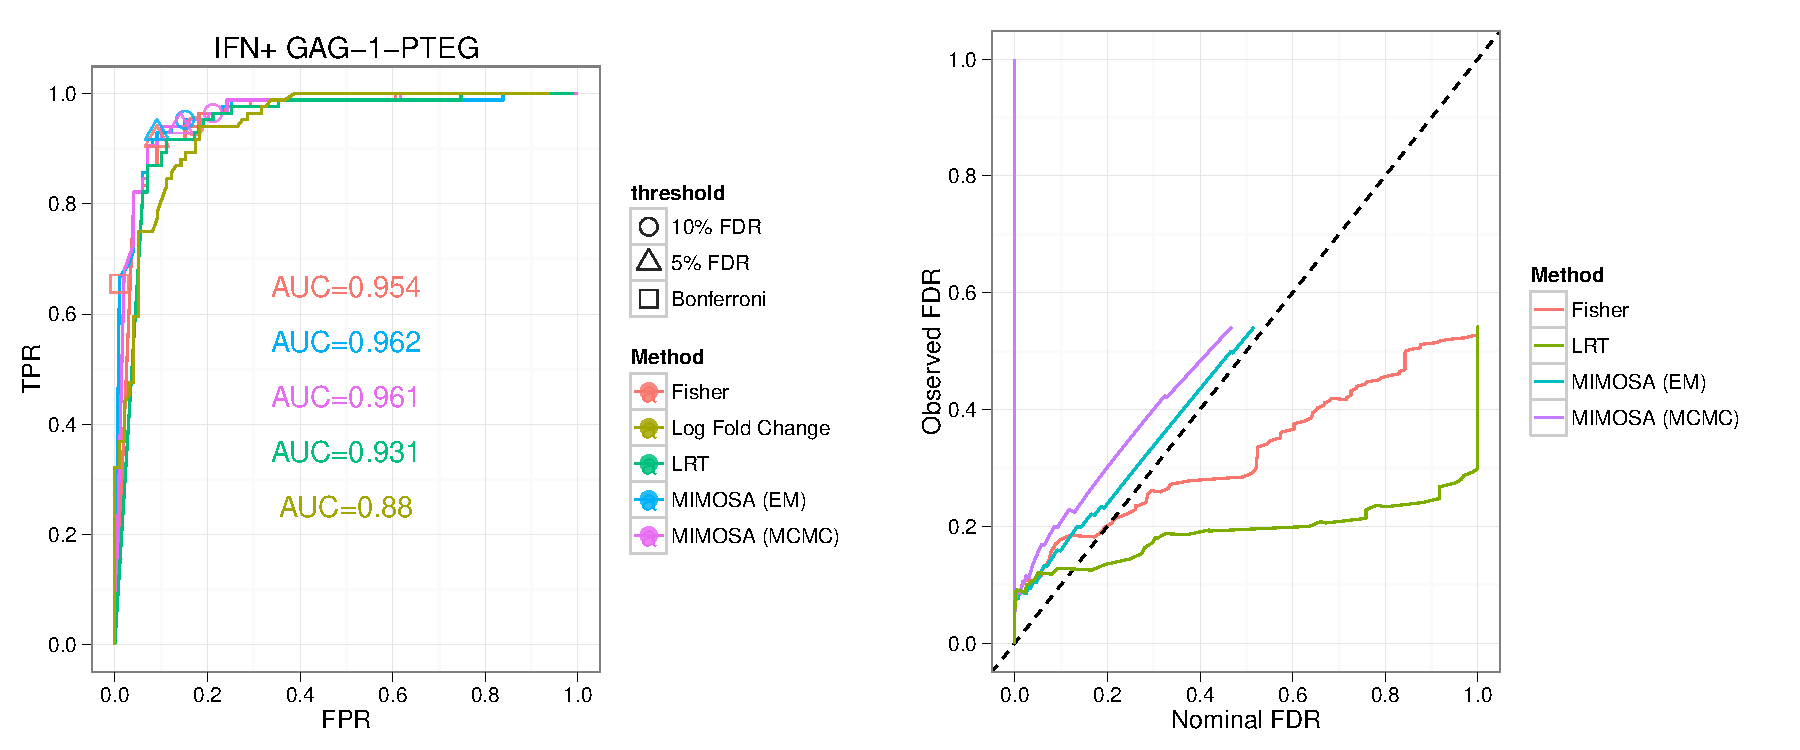
\includegraphics[width=.5\columnwidth]{Figures/9}};
    %\node[anchor=south west, inner sep=0] at (8,-11.25){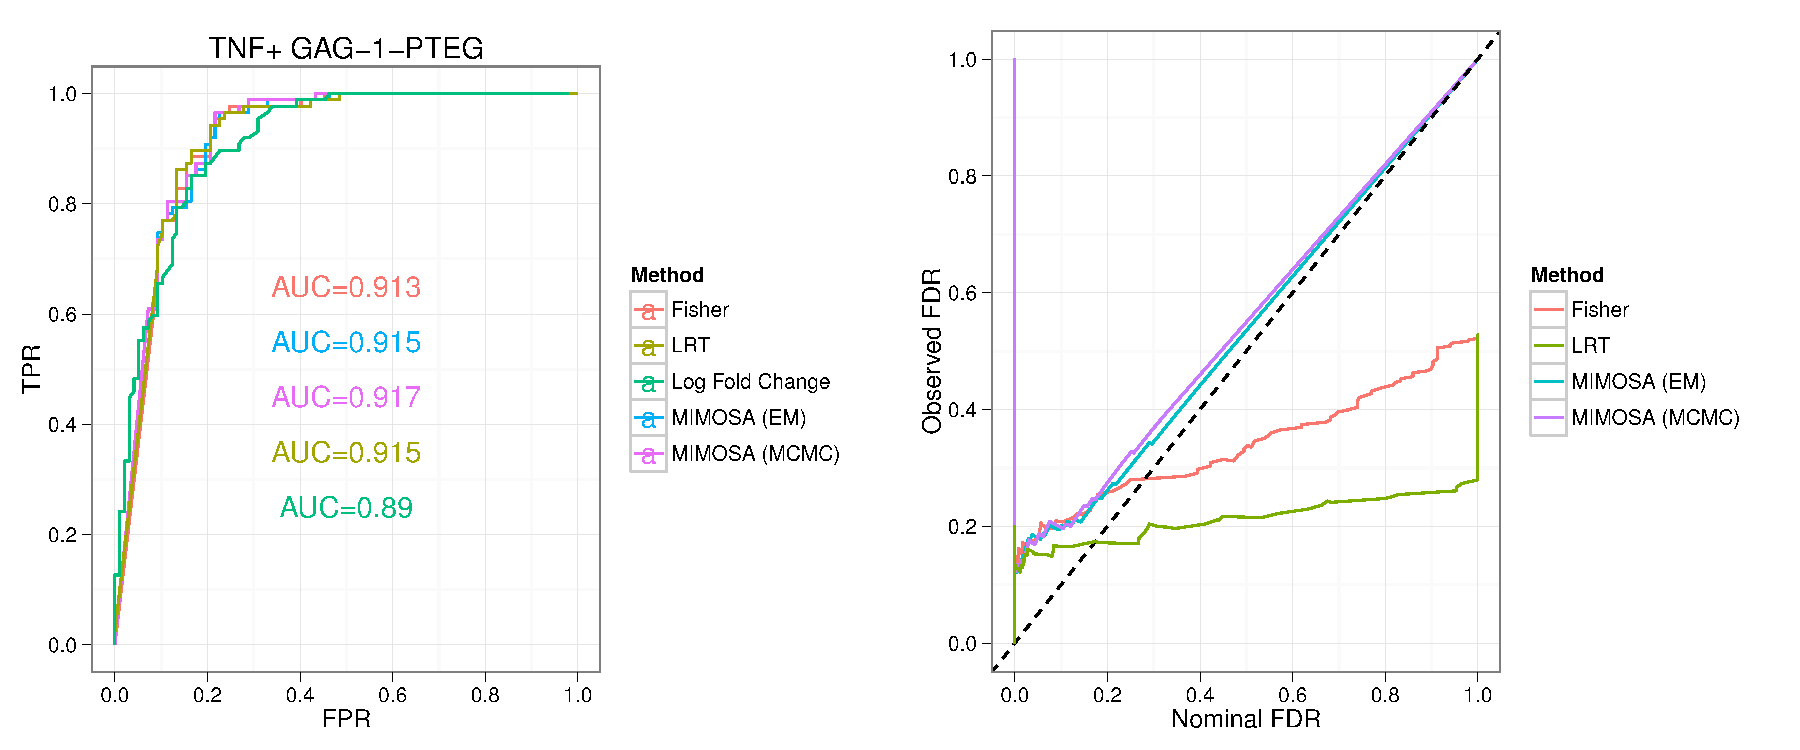
\includegraphics[width=.5\columnwidth]{Figures/10}};
    %\node[anchor=south west, inner sep=0] at (0,-15){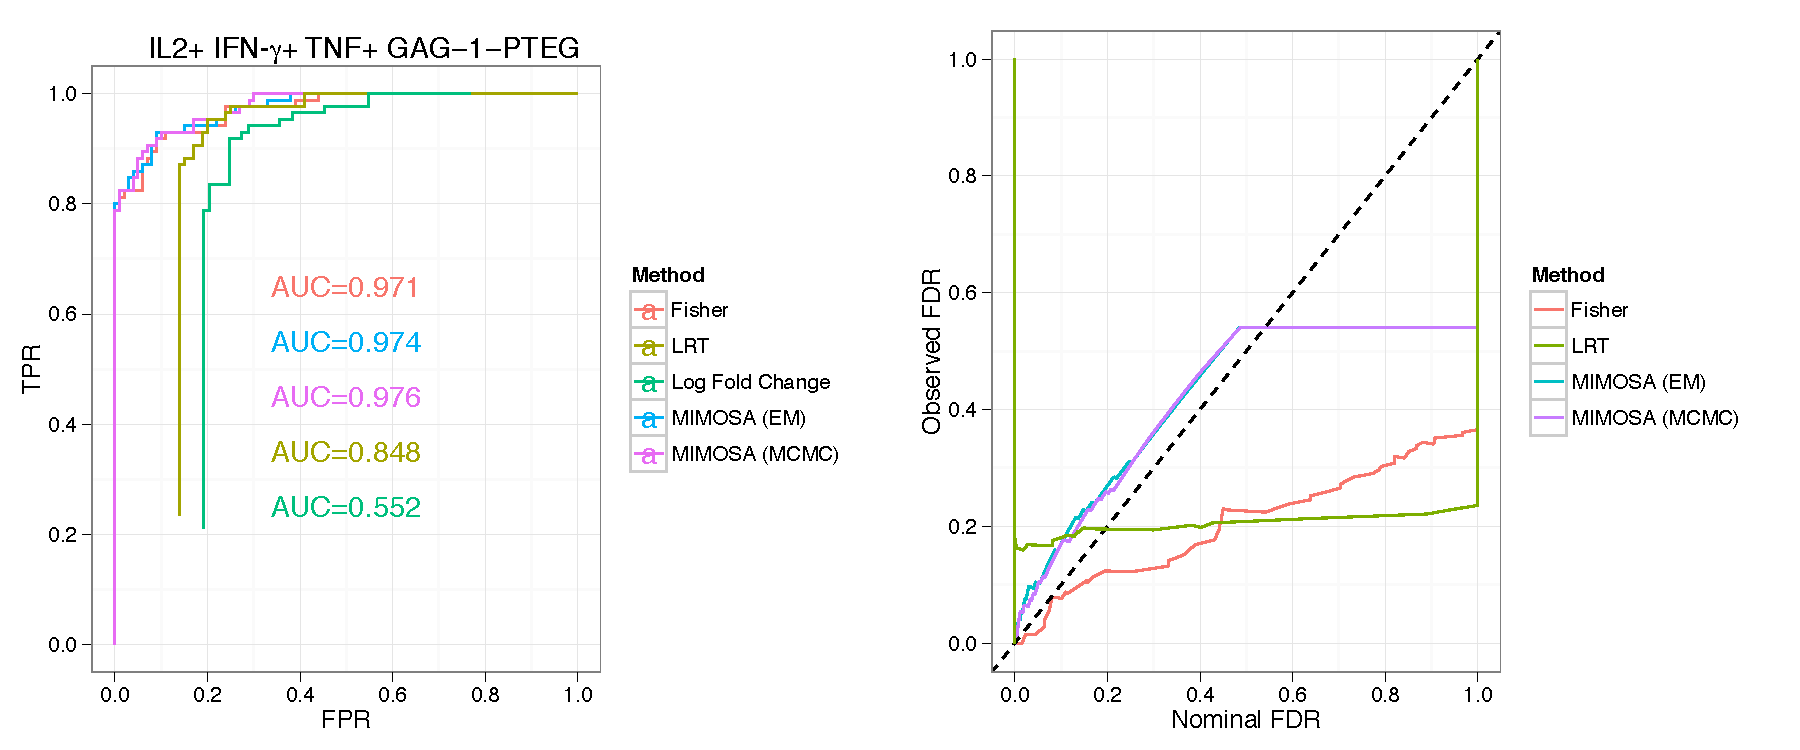
\includegraphics[width=.5\columnwidth]{Figures/11}};
    %\node[anchor=south west, inner sep=0] at (8,-15){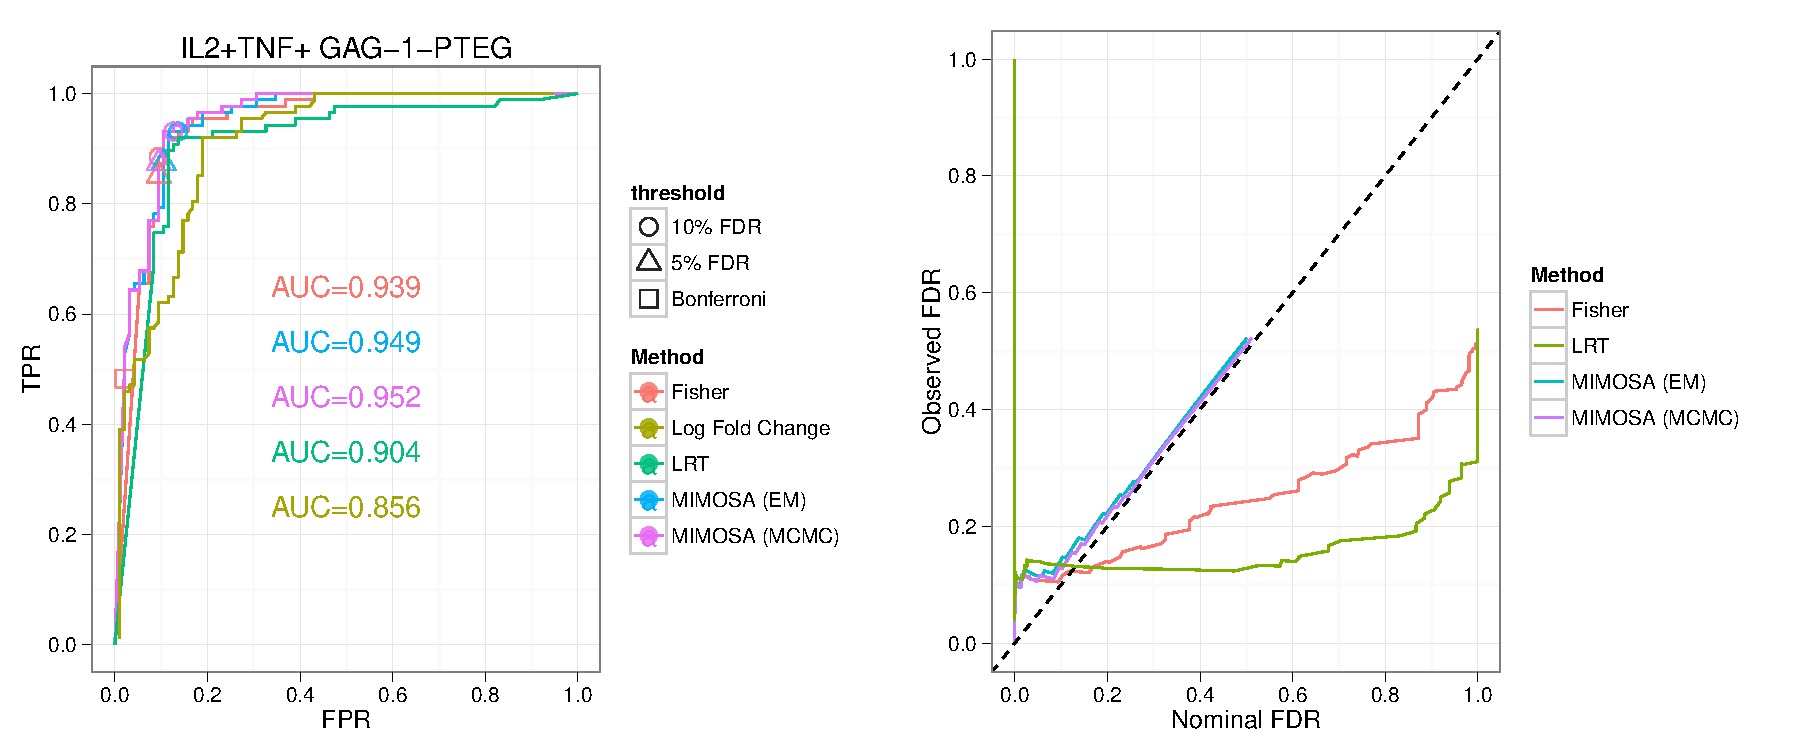
\includegraphics[width=.5\columnwidth]{Figures/13}};

  %  \node at (8,-4) [font=\small\sffamily] {F} ;
%    \node at (0,-7.75) [font=\small\sffamily] {G} ;
  %  \node at (8,-7.75) [font=\small\sffamily] {H} ;
   % \node at (0,-11.75) [font=\small\sffamily] {I} ;
   % \node at (8,-11.75) [font=\small\sffamily] {J} ;
    \end{tikzpicture}
   \caption{Comparison of MIMOSA on other cytokines and cytokine combinations for ENV-1-PTEG stimulated CD4+ T-cells from the HVTN065 trial.}
\label{webfig:HVTN065Results}
\end{figure}

%\begin{figure}[htbp] %  figure placement: here, top, bottom, or page
%   \centering
%%   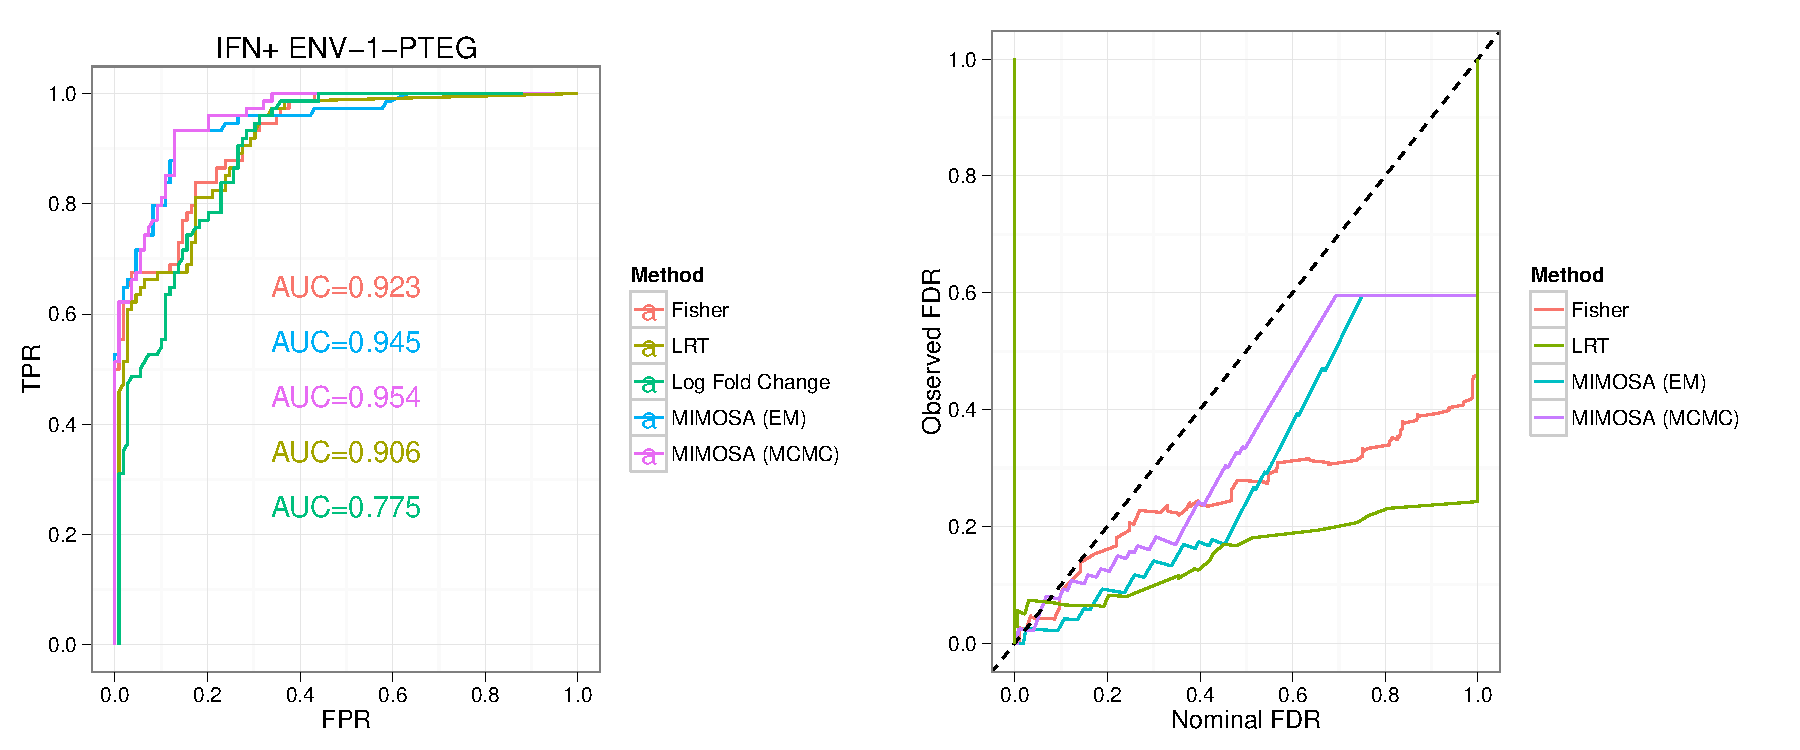
\includegraphics[width=.75\columnwidth]{Figures/2}\\ 
%%   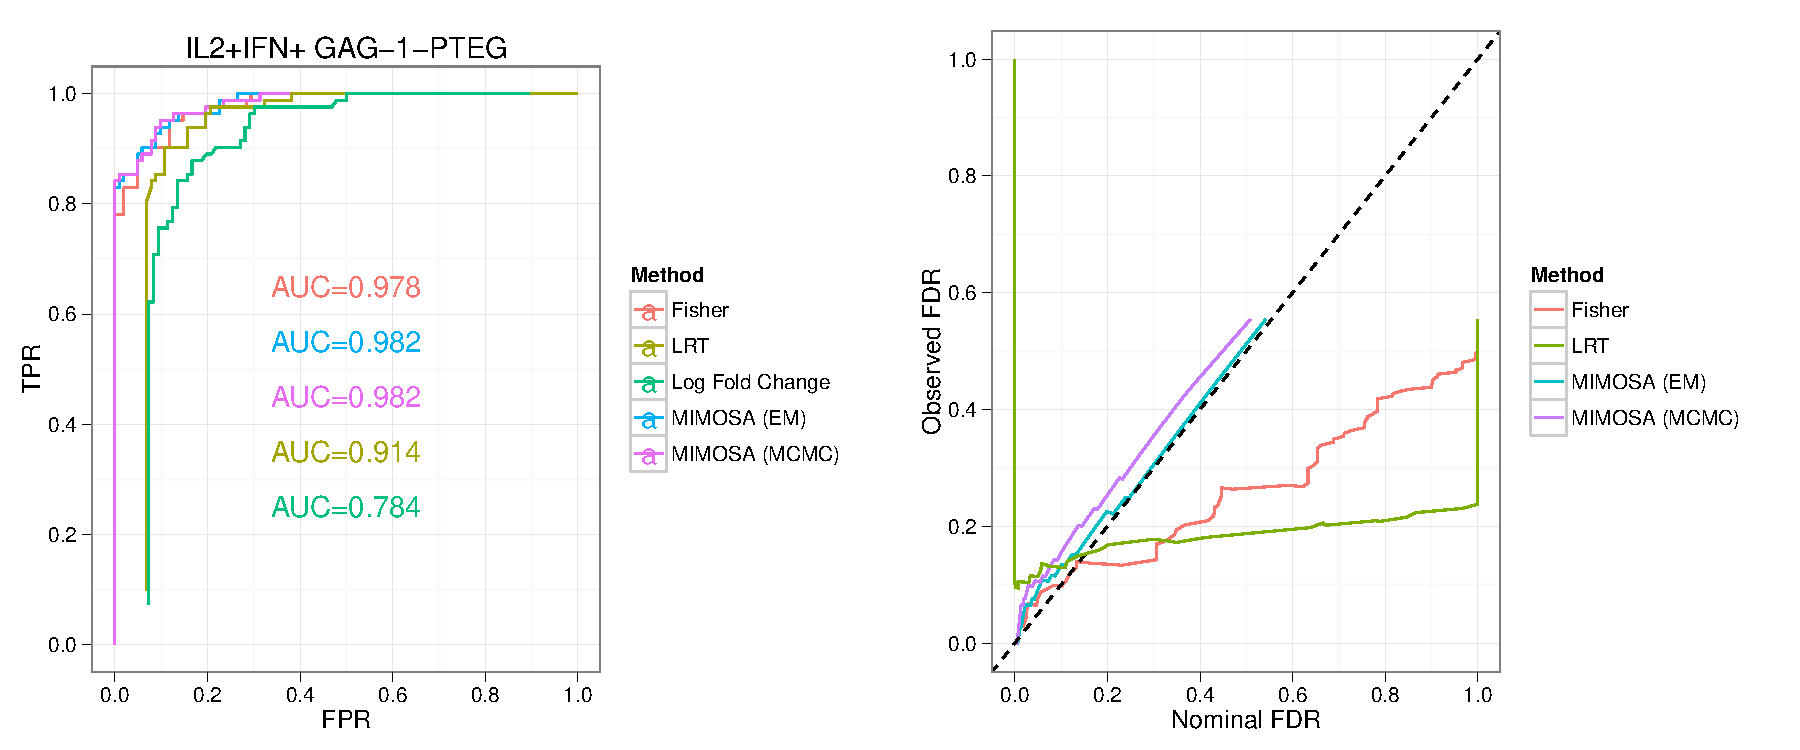
\includegraphics[width=.75\columnwidth]{Figures/12} 
%\begin{tikzpicture}
%    \node[anchor=south west, inner sep=0] at (0,0){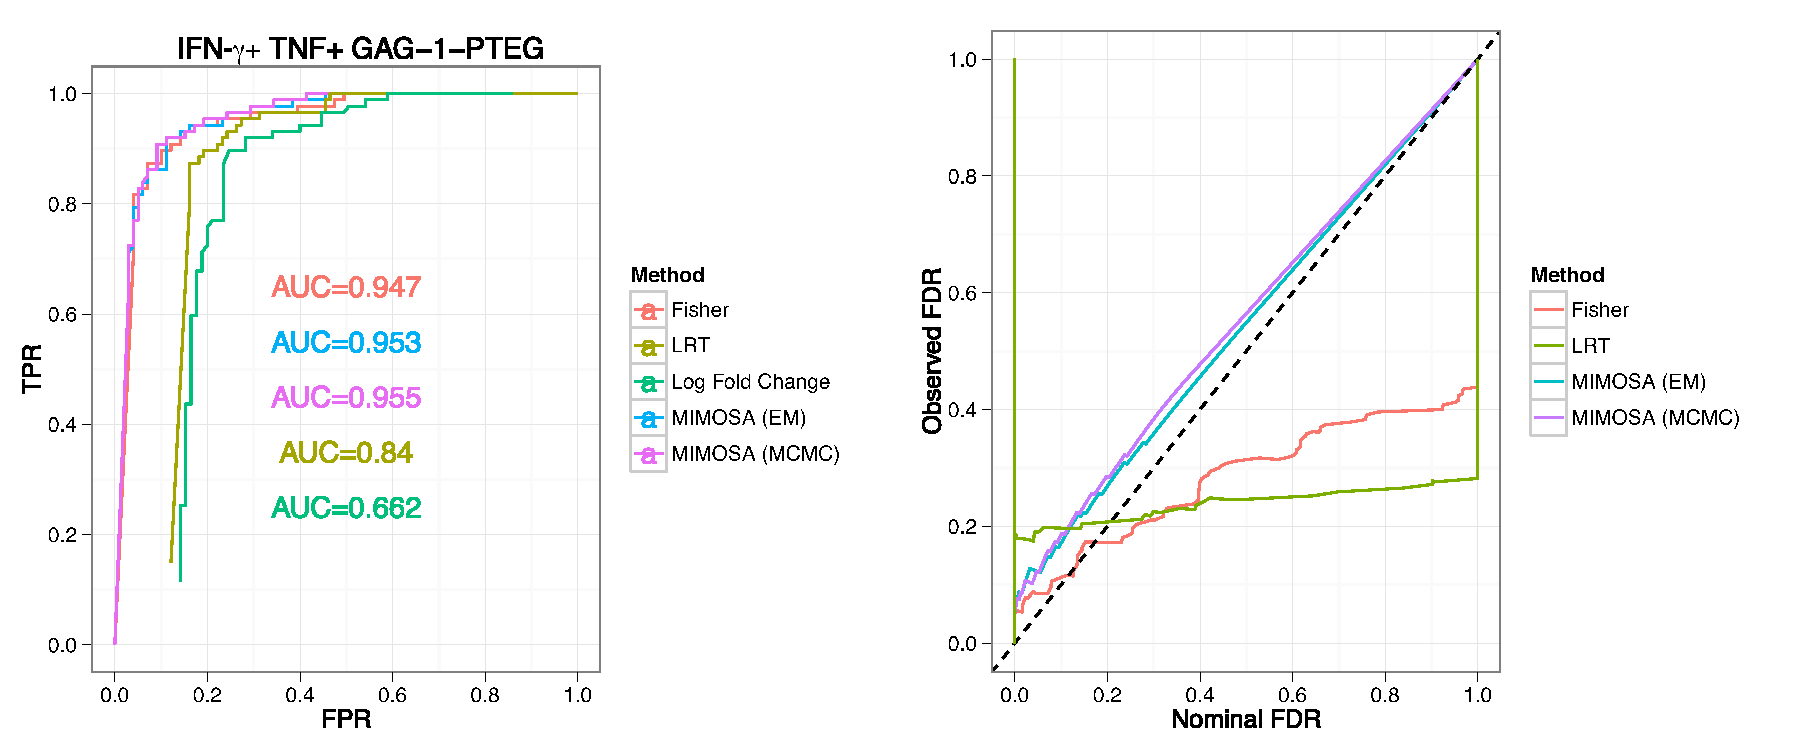
\includegraphics[width=.5\columnwidth]{Figures/14}};
%    \node[anchor=south west, inner sep=0] at (8,0){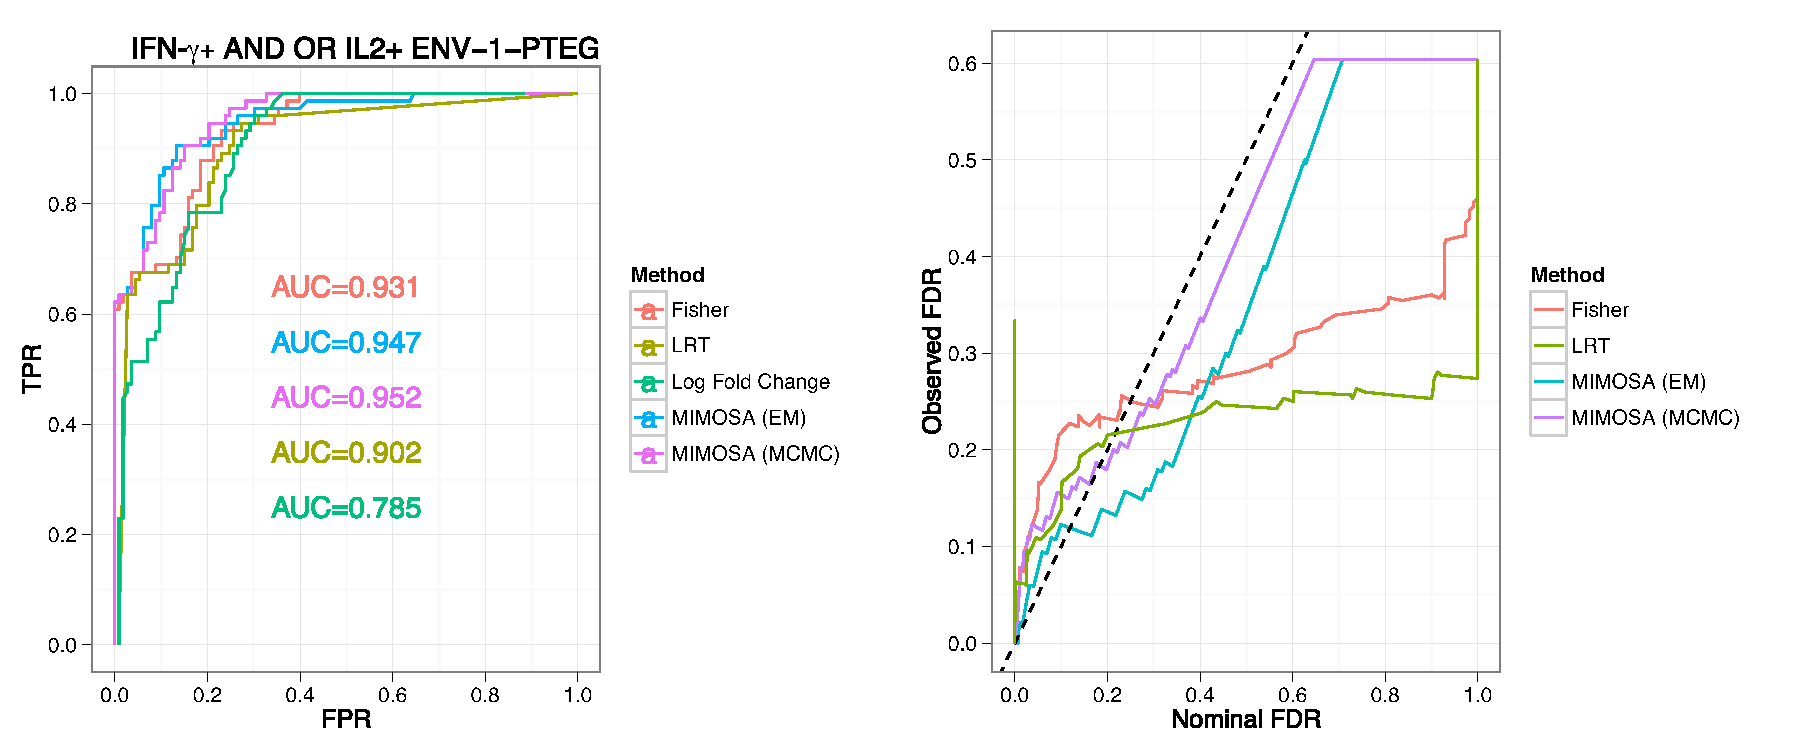
\includegraphics[width=.5\columnwidth]{Figures/15}};
%    \node[anchor=south west, inner sep=0] at (0,-3.75){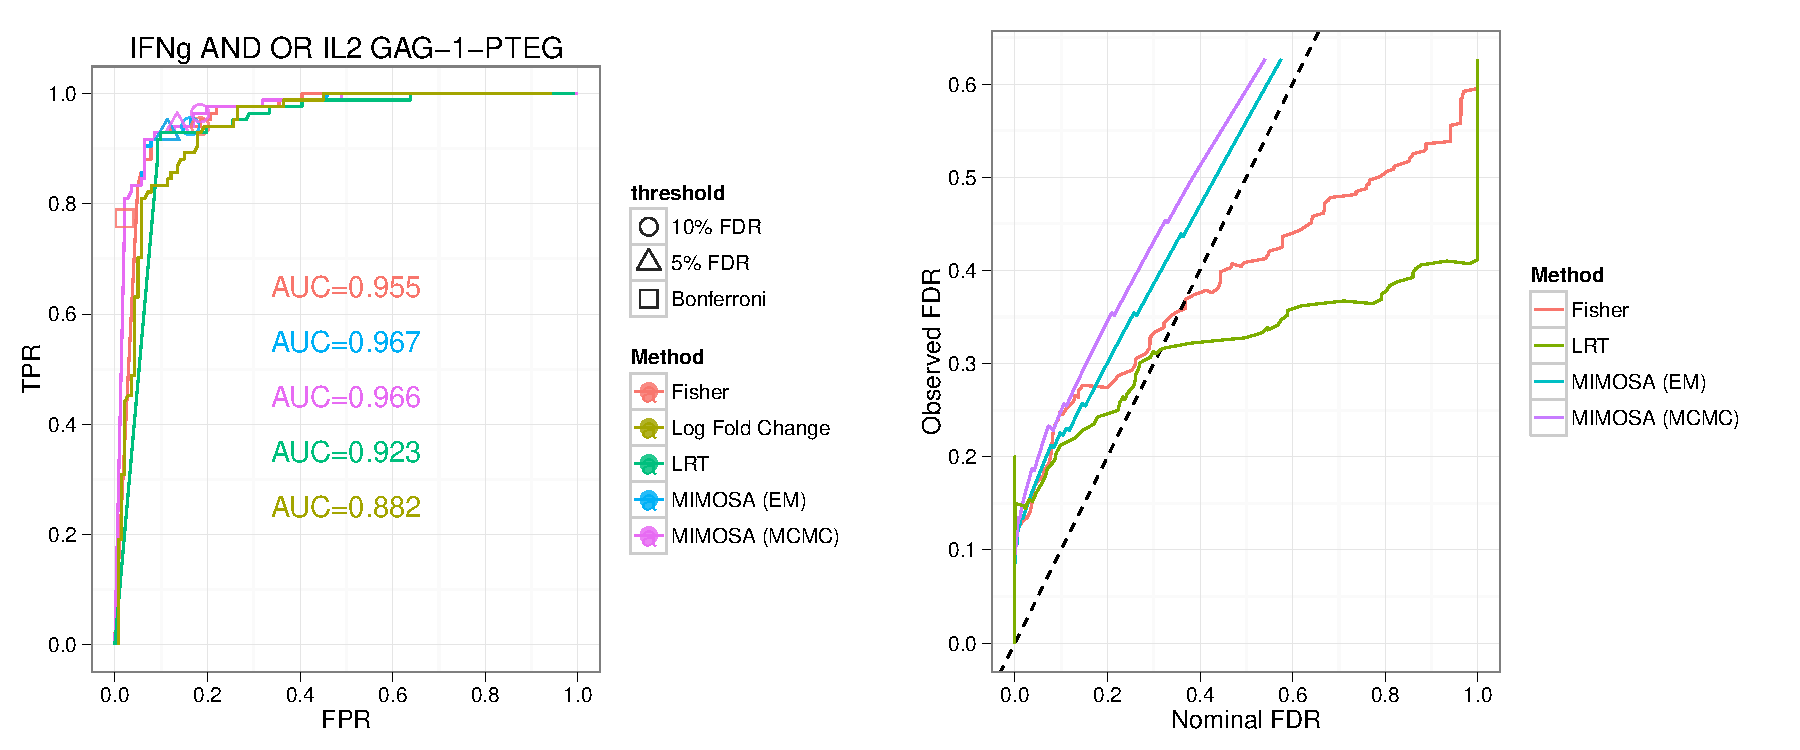
\includegraphics[width=.5\columnwidth]{Figures/16}};
%
%
%    \node at (0,3.4) [font=\small\sffamily] {A} ;
%    \node at (8,3.4) [font=\small\sffamily] {B} ;
%    \node at (0,-0.5) [font=\small\sffamily] {C} ;
%    \end{tikzpicture}
%   \caption{Comparison of MIMOSA on other cytokines and cytokine combinations for ENV-1-PTEG and GAG-1-PTEG stimulated CD4+ T-cells from the HVTN065 trial.}
%\label{fig:HVTN065ResultsCont}
%\end{figure}

\begin{figure} %  figure placement: here, top, bottom, or page
   \centering
\begin{tikzpicture} [auto,node distance=0cm]
%\node at (0,0) (A) {
%\begin{tikzpicture}
%    \node[anchor=south west,inner sep=0] at (0,0) (a) {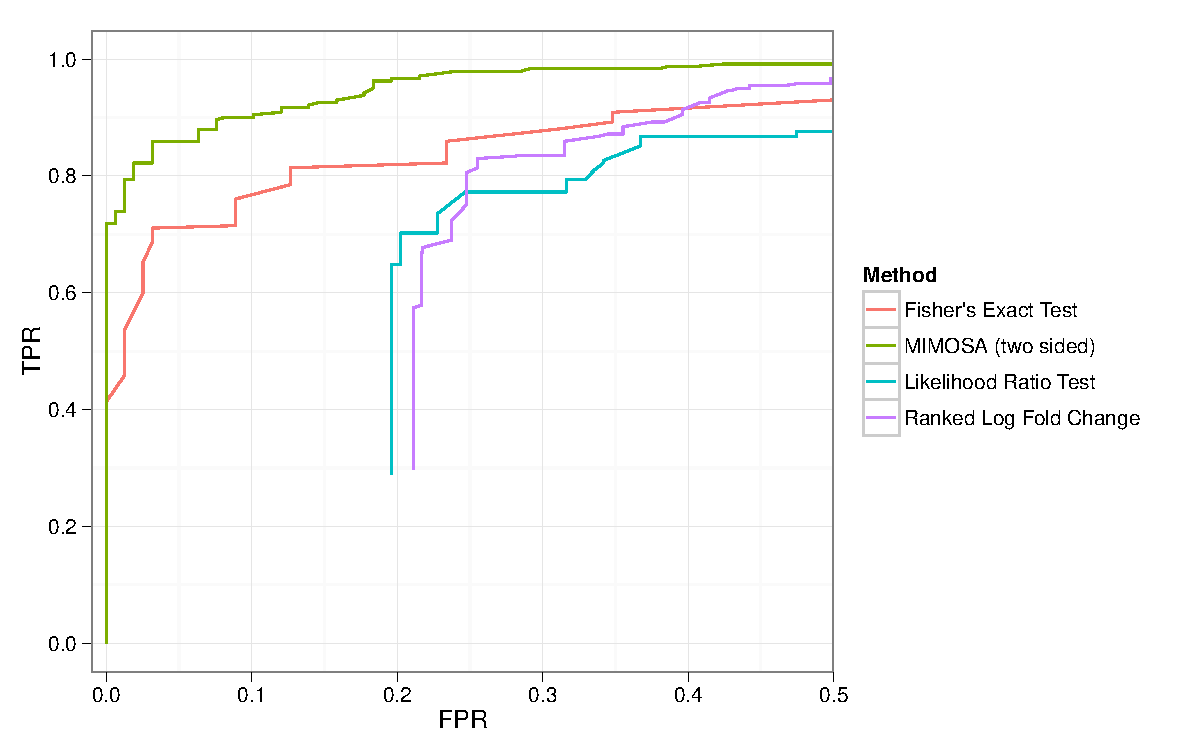
\includegraphics[width=0.4\columnwidth]{Figures/Sim_Twosided_ROC_5000.pdf}};
%    \begin{scope} [x={(a.south east)},y={(a.north west)}]
%        \node at (0,1) [font=\small\sffamily] {A} ;
%    \end{scope}
%    \end{tikzpicture}
%    };
%    \node [right=of A] (B) {
%    \begin{tikzpicture}
%    \node[anchor=south west, inner sep=0] at (0,0) (b) {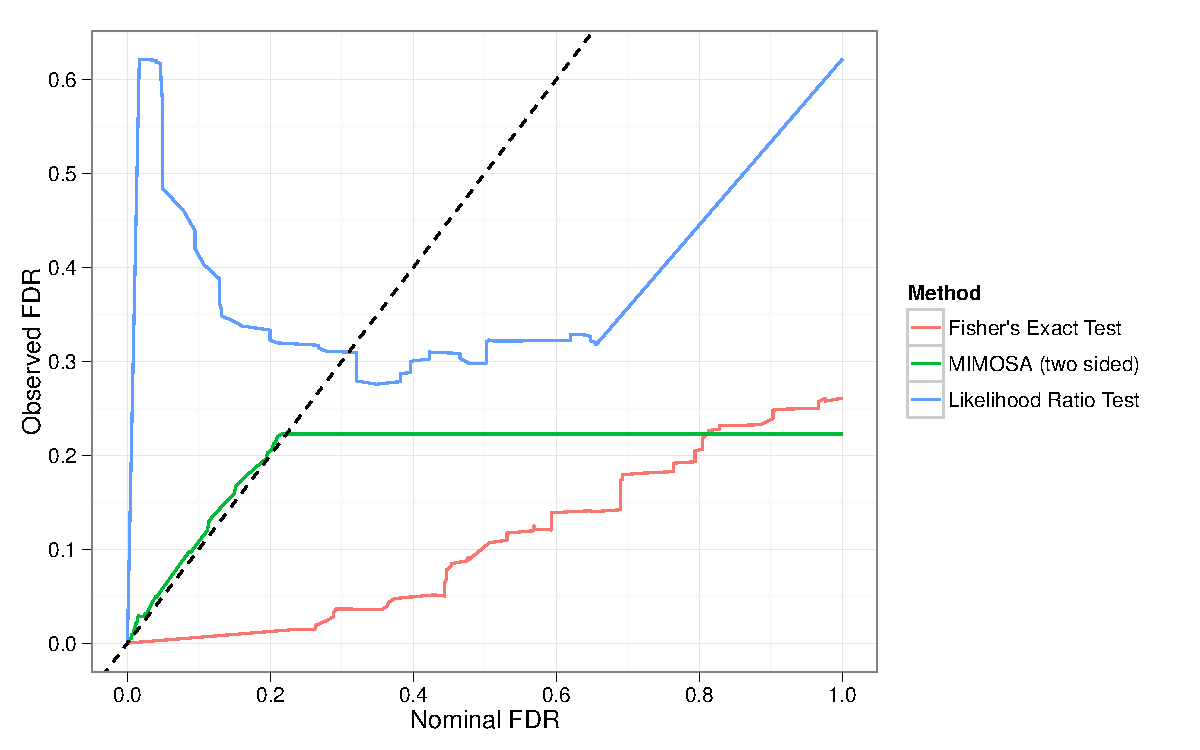
\includegraphics[width=0.4\columnwidth]{Figures/Sim_Twosided_FDR_5000.pdf}};
%        \begin{scope} [x={(b.south east)},y={(b.north west)}]
%        \node at (0,1) [font=\small\sffamily] {B} ;
%        \end{scope}
%    \end{tikzpicture}
%    };
    \node at (0,0) (A) {
    \begin{tikzpicture}
     \node[anchor=south west,inner sep=0] at (0,0) (c) {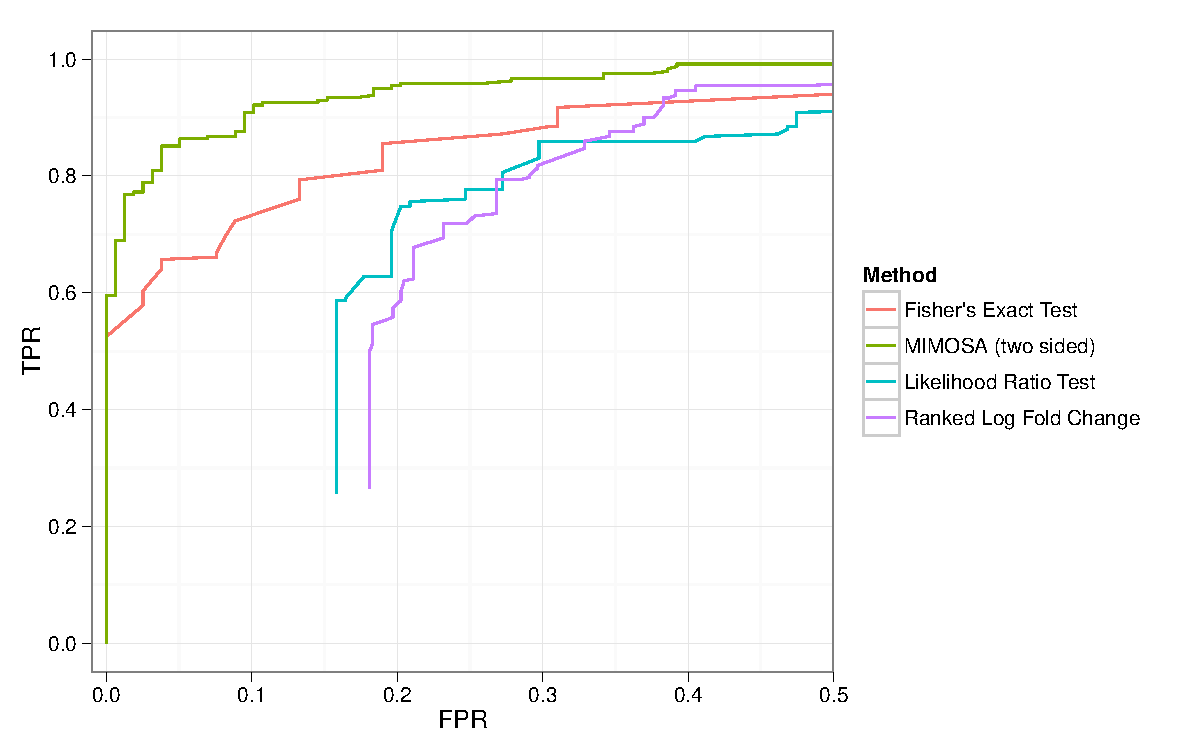
\includegraphics[width=0.4\columnwidth]{Figures/Sim_Truncated_ROC_5000.pdf}};
         \begin{scope} [x={(c.south east)},y={(c.north west)}]
                 \node at (0,1) [font=\small\sffamily] {A} ;
	\end{scope}
     \end{tikzpicture}
     };
     \node [right=of A] (B) {
     \begin{tikzpicture}
    \node[anchor=south west, inner sep=0] at (0,0) (d) {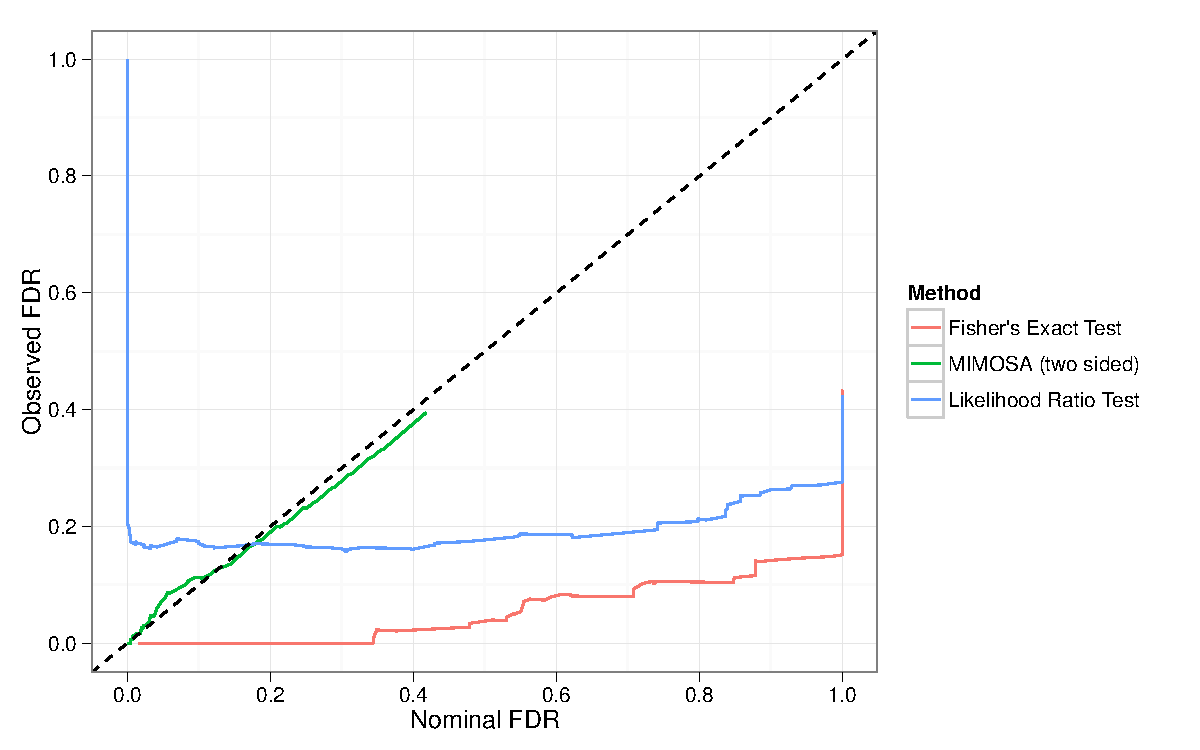
\includegraphics[width=0.4\columnwidth]{Figures/Sim_Truncated_FDR_5000.pdf}};
        \begin{scope} [x={(d.south east)},y={(d.north west)}]
            \node at (0,1) [font=\small\sffamily] {B} ;
\end{scope}
    \end{tikzpicture}
    };
  \node [below=of A] (C) {
\begin{tikzpicture}
    \node[anchor=south west,inner sep=0] at (0,0) (e) {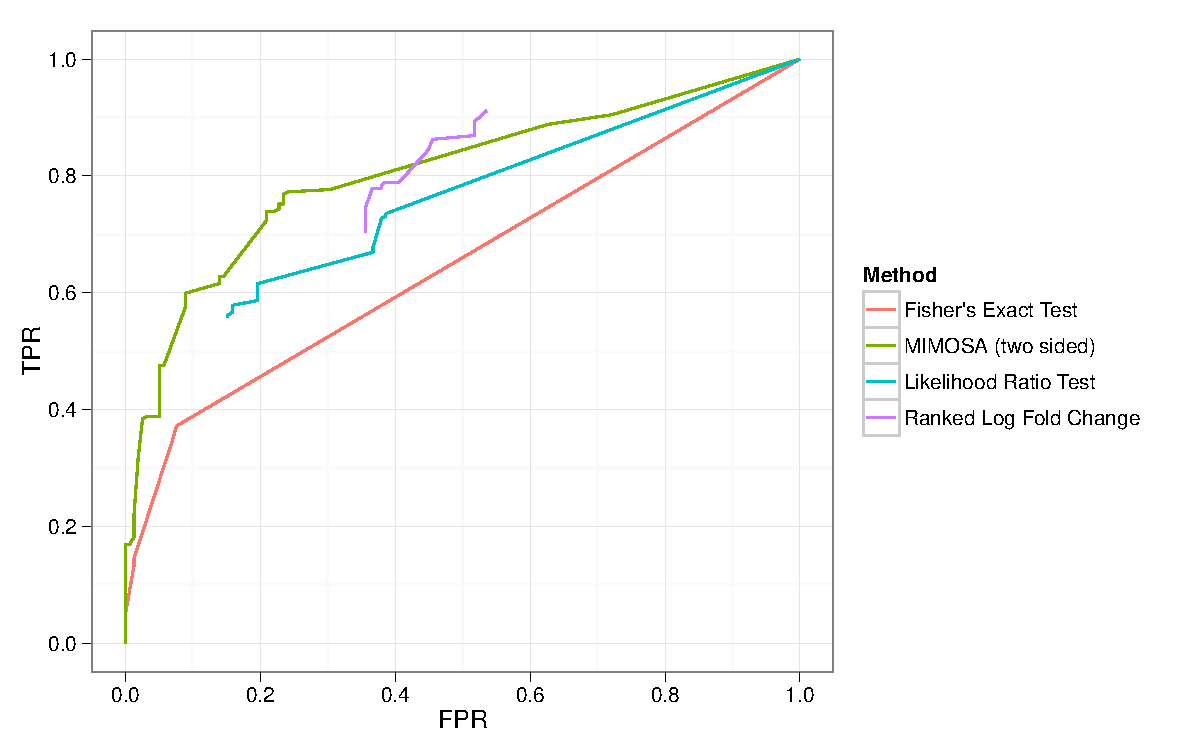
\includegraphics[width=0.4\columnwidth]{Figures/Sim_Truncated_ROC_1000.pdf}};
    \begin{scope} [x={(e.south east)},y={(e.north west)}]
        \node at (0,1) [font=\small\sffamily] {C} ;
    \end{scope}
    \end{tikzpicture}
    };
    \node [right=of C] (D) {
    \begin{tikzpicture}
    \node[anchor=south west, inner sep=0] at (0,0) (f) {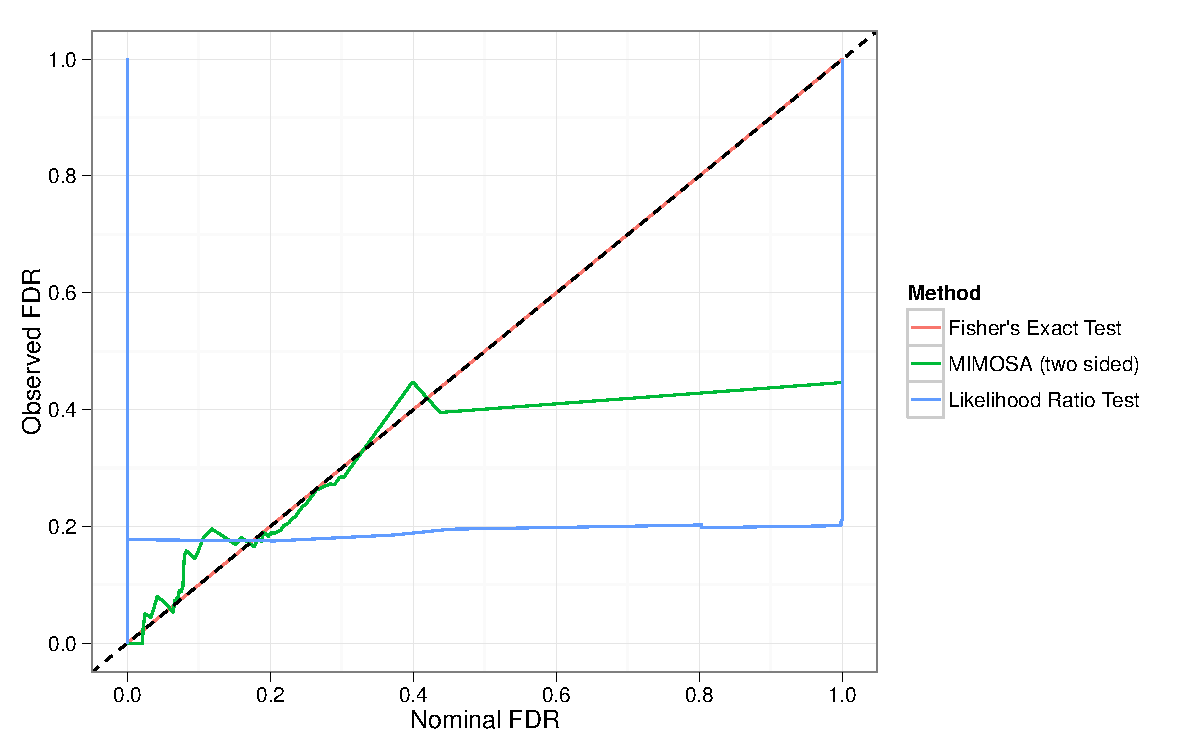
\includegraphics[width=0.4\columnwidth]{Figures/Sim_Truncated_FDR_1000.pdf}};
        \begin{scope} [x={(f.south east)},y={(f.north west)}]
        \node at (0,1) [font=\small\sffamily] {D} ;
        \end{scope}
    \end{tikzpicture}
    };
    \node [below=of C] (E) {
    \begin{tikzpicture}
     \node[anchor=south west,inner sep=0] at (0,0) (g) {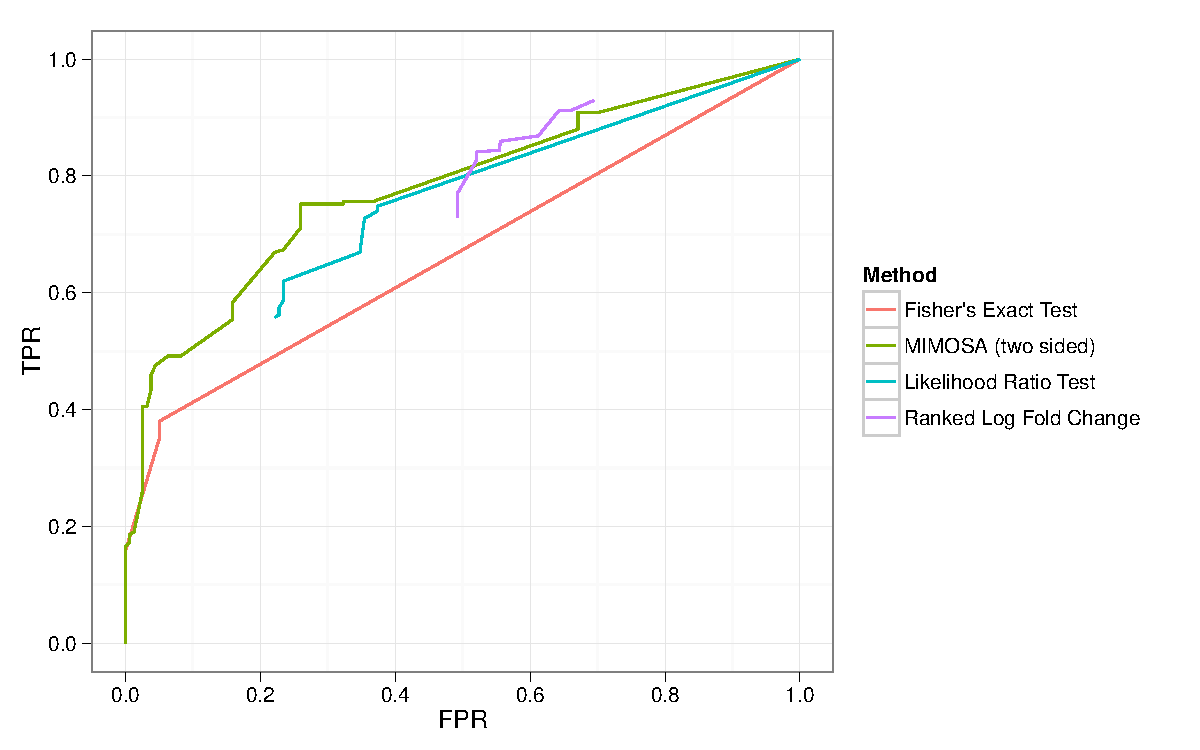
\includegraphics[width=0.4\columnwidth]{Figures/Sim_Twosided_ROC_1000.pdf}};
         \begin{scope} [x={(g.south east)},y={(g.north west)}]
                 \node at (0,1) [font=\small\sffamily] {E} ;
	\end{scope}
     \end{tikzpicture}
     };
     \node [right=of E] (F) {
     \begin{tikzpicture}
    \node[anchor=south west, inner sep=0] at (0,0) (h) {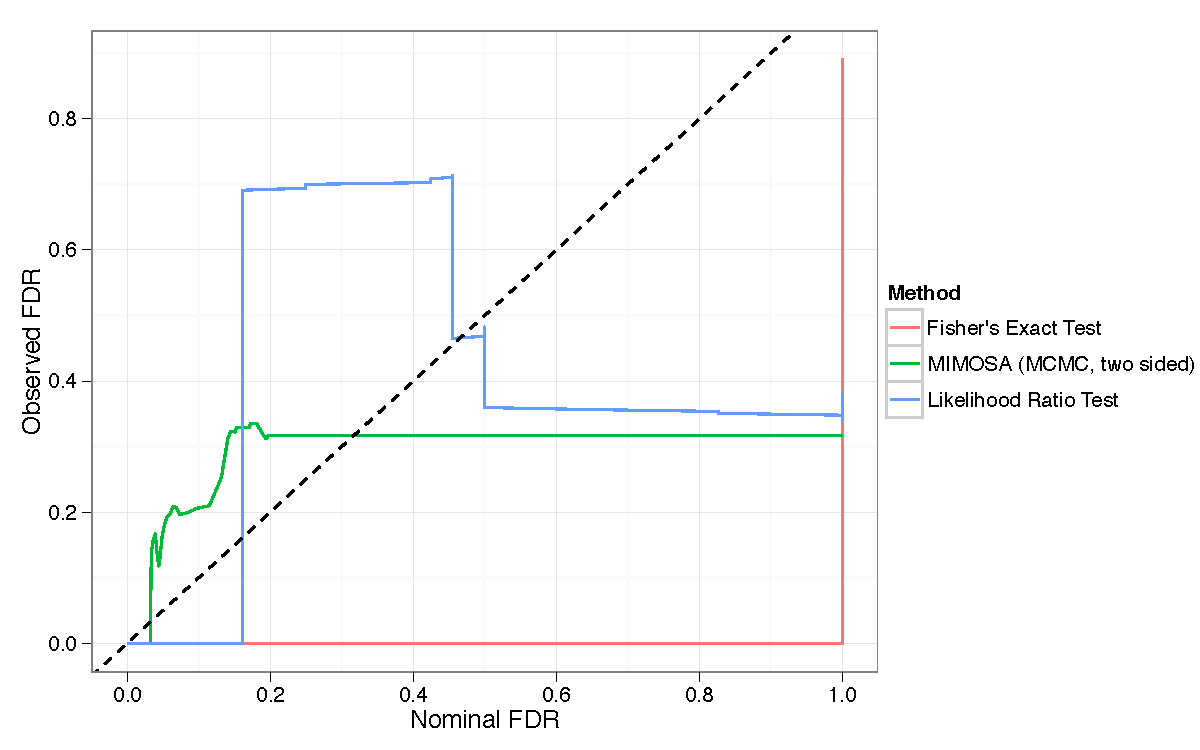
\includegraphics[width=0.4\columnwidth]{Figures/Sim_Twosided_FDR_1000.pdf}};
        \begin{scope} [x={(h.south east)},y={(h.north west)}]
            \node at (0,1) [font=\small\sffamily] {F} ;
\end{scope}
    \end{tikzpicture}
    };
 \end{tikzpicture}
   \caption{Unconstrained MIMOSA model fit to data from a model violating model assumptions and to two--sided data with small counts. Data was simulated from a model where proportions were sampled from a truncated normal distribution over $[0,1]$ rather than a Beta distribution.  A) The average ROC from 10 simulation with N=5,000 events. B) The average observed and nominal FDR from 10 simulations with N=5,000 events. C) Average ROC for N=1,000 events D) Average observed and nominal FDR for N=1,000 events. MIMOSA fit to two--sided data were simulated from the standard model with N=1,000 events. E) Average ROC curves from 10 simulations and F) average observed vs nominal FDR from 10 simulations.}
   \label{webfig:simulations_trunc}
\end{figure}
\bibliographystyle{mn2e}
\bibliography{MIMOSA}


\end{document}